% Options for packages loaded elsewhere
\PassOptionsToPackage{unicode,linktoc=all}{hyperref}
\PassOptionsToPackage{hyphens}{url}
\PassOptionsToPackage{dvipsnames,svgnames,x11names}{xcolor}
%
\documentclass[
  11pt,
  a4paper,
  oneside]{scrbook}

\usepackage{amsmath,amssymb}
\usepackage{iftex}
\ifPDFTeX
  \usepackage[T1]{fontenc}
  \usepackage[utf8]{inputenc}
  \usepackage{textcomp} % provide euro and other symbols
\else % if luatex or xetex
  \usepackage{unicode-math}
  \defaultfontfeatures{Scale=MatchLowercase}
  \defaultfontfeatures[\rmfamily]{Ligatures=TeX,Scale=1}
\fi
\usepackage{lmodern}
\ifPDFTeX\else  
    % xetex/luatex font selection
    \setmainfont[]{Latin Modern Roman}
\fi
% Use upquote if available, for straight quotes in verbatim environments
\IfFileExists{upquote.sty}{\usepackage{upquote}}{}
\IfFileExists{microtype.sty}{% use microtype if available
  \usepackage[]{microtype}
  \UseMicrotypeSet[protrusion]{basicmath} % disable protrusion for tt fonts
}{}
\makeatletter
\@ifundefined{KOMAClassName}{% if non-KOMA class
  \IfFileExists{parskip.sty}{%
    \usepackage{parskip}
  }{% else
    \setlength{\parindent}{0pt}
    \setlength{\parskip}{6pt plus 2pt minus 1pt}}
}{% if KOMA class
  \KOMAoptions{parskip=half}}
\makeatother
\usepackage{xcolor}
\usepackage[top=2.5cm,bottom=2.5cm,left=3cm,right=1.5cm,ignorehead,heightrounded]{geometry}
\setlength{\emergencystretch}{3em} % prevent overfull lines
\setcounter{secnumdepth}{2}
% Make \paragraph and \subparagraph free-standing
\makeatletter
\ifx\paragraph\undefined\else
  \let\oldparagraph\paragraph
  \renewcommand{\paragraph}{
    \@ifstar
      \xxxParagraphStar
      \xxxParagraphNoStar
  }
  \newcommand{\xxxParagraphStar}[1]{\oldparagraph*{#1}\mbox{}}
  \newcommand{\xxxParagraphNoStar}[1]{\oldparagraph{#1}\mbox{}}
\fi
\ifx\subparagraph\undefined\else
  \let\oldsubparagraph\subparagraph
  \renewcommand{\subparagraph}{
    \@ifstar
      \xxxSubParagraphStar
      \xxxSubParagraphNoStar
  }
  \newcommand{\xxxSubParagraphStar}[1]{\oldsubparagraph*{#1}\mbox{}}
  \newcommand{\xxxSubParagraphNoStar}[1]{\oldsubparagraph{#1}\mbox{}}
\fi
\makeatother

\usepackage{color}
\usepackage{fancyvrb}
\newcommand{\VerbBar}{|}
\newcommand{\VERB}{\Verb[commandchars=\\\{\}]}
\DefineVerbatimEnvironment{Highlighting}{Verbatim}{commandchars=\\\{\}}
% Add ',fontsize=\small' for more characters per line
\newenvironment{Shaded}{}{}
\newcommand{\AlertTok}[1]{\textcolor[rgb]{1.00,0.33,0.33}{\textbf{#1}}}
\newcommand{\AnnotationTok}[1]{\textcolor[rgb]{0.42,0.45,0.49}{#1}}
\newcommand{\AttributeTok}[1]{\textcolor[rgb]{0.84,0.23,0.29}{#1}}
\newcommand{\BaseNTok}[1]{\textcolor[rgb]{0.00,0.36,0.77}{#1}}
\newcommand{\BuiltInTok}[1]{\textcolor[rgb]{0.84,0.23,0.29}{#1}}
\newcommand{\CharTok}[1]{\textcolor[rgb]{0.01,0.18,0.38}{#1}}
\newcommand{\CommentTok}[1]{\textcolor[rgb]{0.42,0.45,0.49}{#1}}
\newcommand{\CommentVarTok}[1]{\textcolor[rgb]{0.42,0.45,0.49}{#1}}
\newcommand{\ConstantTok}[1]{\textcolor[rgb]{0.00,0.36,0.77}{#1}}
\newcommand{\ControlFlowTok}[1]{\textcolor[rgb]{0.84,0.23,0.29}{#1}}
\newcommand{\DataTypeTok}[1]{\textcolor[rgb]{0.84,0.23,0.29}{#1}}
\newcommand{\DecValTok}[1]{\textcolor[rgb]{0.00,0.36,0.77}{#1}}
\newcommand{\DocumentationTok}[1]{\textcolor[rgb]{0.42,0.45,0.49}{#1}}
\newcommand{\ErrorTok}[1]{\textcolor[rgb]{1.00,0.33,0.33}{\underline{#1}}}
\newcommand{\ExtensionTok}[1]{\textcolor[rgb]{0.84,0.23,0.29}{\textbf{#1}}}
\newcommand{\FloatTok}[1]{\textcolor[rgb]{0.00,0.36,0.77}{#1}}
\newcommand{\FunctionTok}[1]{\textcolor[rgb]{0.44,0.26,0.76}{#1}}
\newcommand{\ImportTok}[1]{\textcolor[rgb]{0.01,0.18,0.38}{#1}}
\newcommand{\InformationTok}[1]{\textcolor[rgb]{0.42,0.45,0.49}{#1}}
\newcommand{\KeywordTok}[1]{\textcolor[rgb]{0.84,0.23,0.29}{#1}}
\newcommand{\NormalTok}[1]{\textcolor[rgb]{0.14,0.16,0.18}{#1}}
\newcommand{\OperatorTok}[1]{\textcolor[rgb]{0.14,0.16,0.18}{#1}}
\newcommand{\OtherTok}[1]{\textcolor[rgb]{0.44,0.26,0.76}{#1}}
\newcommand{\PreprocessorTok}[1]{\textcolor[rgb]{0.84,0.23,0.29}{#1}}
\newcommand{\RegionMarkerTok}[1]{\textcolor[rgb]{0.42,0.45,0.49}{#1}}
\newcommand{\SpecialCharTok}[1]{\textcolor[rgb]{0.00,0.36,0.77}{#1}}
\newcommand{\SpecialStringTok}[1]{\textcolor[rgb]{0.01,0.18,0.38}{#1}}
\newcommand{\StringTok}[1]{\textcolor[rgb]{0.01,0.18,0.38}{#1}}
\newcommand{\VariableTok}[1]{\textcolor[rgb]{0.89,0.38,0.04}{#1}}
\newcommand{\VerbatimStringTok}[1]{\textcolor[rgb]{0.01,0.18,0.38}{#1}}
\newcommand{\WarningTok}[1]{\textcolor[rgb]{1.00,0.33,0.33}{#1}}

\providecommand{\tightlist}{%
  \setlength{\itemsep}{0pt}\setlength{\parskip}{0pt}}\usepackage{longtable,booktabs,array}
\usepackage{calc} % for calculating minipage widths
% Correct order of tables after \paragraph or \subparagraph
\usepackage{etoolbox}
\makeatletter
\patchcmd\longtable{\par}{\if@noskipsec\mbox{}\fi\par}{}{}
\makeatother
% Allow footnotes in longtable head/foot
\IfFileExists{footnotehyper.sty}{\usepackage{footnotehyper}}{\usepackage{footnote}}
\makesavenoteenv{longtable}
\usepackage{graphicx}
\makeatletter
\newsavebox\pandoc@box
\newcommand*\pandocbounded[1]{% scales image to fit in text height/width
  \sbox\pandoc@box{#1}%
  \Gscale@div\@tempa{\textheight}{\dimexpr\ht\pandoc@box+\dp\pandoc@box\relax}%
  \Gscale@div\@tempb{\linewidth}{\wd\pandoc@box}%
  \ifdim\@tempb\p@<\@tempa\p@\let\@tempa\@tempb\fi% select the smaller of both
  \ifdim\@tempa\p@<\p@\scalebox{\@tempa}{\usebox\pandoc@box}%
  \else\usebox{\pandoc@box}%
  \fi%
}
% Set default figure placement to htbp
\def\fps@figure{htbp}
\makeatother
% definitions for citeproc citations
\NewDocumentCommand\citeproctext{}{}
\NewDocumentCommand\citeproc{mm}{%
  \begingroup\def\citeproctext{#2}\cite{#1}\endgroup}
\makeatletter
 % allow citations to break across lines
 \let\@cite@ofmt\@firstofone
 % avoid brackets around text for \cite:
 \def\@biblabel#1{}
 \def\@cite#1#2{{#1\if@tempswa , #2\fi}}
\makeatother
\newlength{\cslhangindent}
\setlength{\cslhangindent}{1.5em}
\newlength{\csllabelwidth}
\setlength{\csllabelwidth}{3em}
\newenvironment{CSLReferences}[2] % #1 hanging-indent, #2 entry-spacing
 {\begin{list}{}{%
  \setlength{\itemindent}{0pt}
  \setlength{\leftmargin}{0pt}
  \setlength{\parsep}{0pt}
  % turn on hanging indent if param 1 is 1
  \ifodd #1
   \setlength{\leftmargin}{\cslhangindent}
   \setlength{\itemindent}{-1\cslhangindent}
  \fi
  % set entry spacing
  \setlength{\itemsep}{#2\baselineskip}}}
 {\end{list}}
\usepackage{calc}
\newcommand{\CSLBlock}[1]{\hfill\break\parbox[t]{\linewidth}{\strut\ignorespaces#1\strut}}
\newcommand{\CSLLeftMargin}[1]{\parbox[t]{\csllabelwidth}{\strut#1\strut}}
\newcommand{\CSLRightInline}[1]{\parbox[t]{\linewidth - \csllabelwidth}{\strut#1\strut}}
\newcommand{\CSLIndent}[1]{\hspace{\cslhangindent}#1}

% ---------- PROFESSOR'S HEADER (KEEP THIS) ----------
\addtokomafont{disposition}{\rmfamily}
\KOMAoptions{chapterprefix=true,appendixprefix=true}
\KOMAoptions{headings=small}

\setkomafont{pageheadfoot}{\normalfont\normalcolor\footnotesize}
\setkomafont{pagenumber}{\normalfont\normalcolor\footnotesize}

\usepackage{scrlayer-scrpage}
\lefoot[]{}
\cefoot[\pagemark]{}
\refoot[]{}
\lofoot[]{}
\cofoot[\pagemark]{}
\rofoot[]{}
\lehead[]{\pagemark}
\cehead[]{}
\rehead[]{\leftmark}
\lohead[]{\rightmark}
\cohead[]{}
\rohead[]{\pagemark}


% ---------- OPTIONAL IMPROVEMENTS ----------
% No blank pages before chapters in pdf
\KOMAoptions{open=any, cleardoublepage=empty}

% Better chapter spacing
\RedeclareSectionCommand[
  beforeskip=-1ex plus -1ex minus -1ex,
  afterskip=2ex plus 1ex minus 1ex
]{chapter}
\makeatletter
\@ifpackageloaded{tcolorbox}{}{\usepackage[skins,breakable]{tcolorbox}}
\@ifpackageloaded{fontawesome5}{}{\usepackage{fontawesome5}}
\definecolor{quarto-callout-color}{HTML}{909090}
\definecolor{quarto-callout-note-color}{HTML}{0758E5}
\definecolor{quarto-callout-important-color}{HTML}{CC1914}
\definecolor{quarto-callout-warning-color}{HTML}{EB9113}
\definecolor{quarto-callout-tip-color}{HTML}{00A047}
\definecolor{quarto-callout-caution-color}{HTML}{FC5300}
\definecolor{quarto-callout-color-frame}{HTML}{acacac}
\definecolor{quarto-callout-note-color-frame}{HTML}{4582ec}
\definecolor{quarto-callout-important-color-frame}{HTML}{d9534f}
\definecolor{quarto-callout-warning-color-frame}{HTML}{f0ad4e}
\definecolor{quarto-callout-tip-color-frame}{HTML}{02b875}
\definecolor{quarto-callout-caution-color-frame}{HTML}{fd7e14}
\makeatother
\makeatletter
\@ifpackageloaded{bookmark}{}{\usepackage{bookmark}}
\makeatother
\makeatletter
\@ifpackageloaded{caption}{}{\usepackage{caption}}
\AtBeginDocument{%
\ifdefined\contentsname
  \renewcommand*\contentsname{Table of contents}
\else
  \newcommand\contentsname{Table of contents}
\fi
\ifdefined\listfigurename
  \renewcommand*\listfigurename{List of Figures}
\else
  \newcommand\listfigurename{List of Figures}
\fi
\ifdefined\listtablename
  \renewcommand*\listtablename{List of Tables}
\else
  \newcommand\listtablename{List of Tables}
\fi
\ifdefined\figurename
  \renewcommand*\figurename{Figure}
\else
  \newcommand\figurename{Figure}
\fi
\ifdefined\tablename
  \renewcommand*\tablename{Table}
\else
  \newcommand\tablename{Table}
\fi
}
\@ifpackageloaded{float}{}{\usepackage{float}}
\floatstyle{ruled}
\@ifundefined{c@chapter}{\newfloat{codelisting}{h}{lop}}{\newfloat{codelisting}{h}{lop}[chapter]}
\floatname{codelisting}{Listing}
\newcommand*\listoflistings{\listof{codelisting}{List of Listings}}
\makeatother
\makeatletter
\makeatother
\makeatletter
\@ifpackageloaded{caption}{}{\usepackage{caption}}
\@ifpackageloaded{subcaption}{}{\usepackage{subcaption}}
\makeatother

\usepackage{bookmark}

\IfFileExists{xurl.sty}{\usepackage{xurl}}{} % add URL line breaks if available
\urlstyle{same} % disable monospaced font for URLs
\hypersetup{
  pdftitle={Assessing the feasibility of developing and taping-out an analog block for LED driver control using IHP-Open-PDK and IIC-OSIC-TOOLS},
  pdfauthor={Priyanka Toyni; Hrishikesh Pangavhane},
  colorlinks=true,
  linkcolor={blue},
  filecolor={Maroon},
  citecolor={Blue},
  urlcolor={Blue},
  pdfcreator={LaTeX via pandoc}}


\title{Assessing the feasibility of developing and taping-out an analog
block for LED driver control using IHP-Open-PDK and IIC-OSIC-TOOLS}
\author{Priyanka Toyni \and Hrishikesh Pangavhane}
\date{November 2025}

\begin{document}
\frontmatter
\maketitle

\begin{titlepage}
\begin{center}

% ------------------------------------------------
% LOGO
% ------------------------------------------------
\vspace*{-1cm}
\includegraphics[width=5.5cm]{figures/hsb-logo.png}

\vspace{0.8cm}

{\large Faculty of Electrical Engineering and Computer Science}

\vspace{1cm}

% ------------------------------------------------
% TITLE
% ------------------------------------------------
{\bfseries\Large
Assessing the feasibility of developing and\\[4pt] taping-out an analog block for LED driver\\[4pt] control using \textbf{IHP-Open-PDK} and\\[4pt] \textbf{IIC-OSIC-TOOLS}
}\\[1cm]




% ------------------------------------------------
% AUTHORS
% ------------------------------------------------
{\large by}\\[10pt]

{\Large Priyanka Toyni}\\
{\large Matr.-Nr.: 5363791}\\[16pt]
{\large ORCID iD: 0009-0007-6435-4990}\\[16pt]

{\Large Hrishikesh Pangavhane}\\
{\large Matr.-Nr.: 5363452}\\[16pt]
{\large ORCID iD: 0009-0008-0089-336X}\\[16pt]

\vspace{1cm}

% ------------------------------------------------
% SUBMISSION INFO
% ------------------------------------------------
{\large A Thesis presented to the City University Bremen\\
in fulfillment of the thesis requirement for the degree of\\
Master in Electronics Engineering}

\vspace{1cm}

% ------------------------------------------------
% EXAMINERS
% ------------------------------------------------
\begin{tabular}{rl}
1. Examiner: & Prof. Dr.-Ing. M. Meiners \\
2. Examiner: & Prof. Dr. (PhD) S. Peik \\
\end{tabular}

\vspace{1cm}

% ------------------------------------------------
% DATES
% ------------------------------------------------
{\large Preparation Period: 26.05.2025 -- 26.11.2025}

\end{center}
\end{titlepage}

% \mainmatter
% \clearpage

\renewcommand*\contentsname{Table of contents}
{
\hypersetup{linkcolor=}
\setcounter{tocdepth}{2}
\tableofcontents
}
\listoffigures
\listoftables

\mainmatter
\bookmarksetup{startatroot}

\chapter*{List of Abbreviations}\label{list-of-abbreviations}

\markboth{List of Abbreviations}{List of Abbreviations}

\textbf{AC} --- Alternating Current\\
\textbf{AVDD} --- Analog Supply Voltage\\
\textbf{AVSS} --- Analog Ground

\textbf{CACE} --- Computer-Aided Circuit Evaluation\\
\textbf{CC} --- Coupling Capacitor\\
\textbf{C} --- Capacitance\\
\textbf{\(C_{gd}\)} --- Gate--Drain Capacitance\\
\textbf{\(C_{gs}\)} --- Gate--Source Capacitance\\
\textbf{CMOS} --- Complementary Metal--Oxide--Semiconductor\\
\textbf{CMRR} --- Common-Mode Rejection Ratio

\textbf{DC} --- Direct Current\\
\textbf{DFM} --- Design for Manufacturability\\
\textbf{DRC} --- Design Rule Check

\textbf{EDA} --- Electronic Design Automation\\
\textbf{EDA-OS} --- Open-Source Electronic Design Automation\\
\textbf{ESD} --- Electrostatic Discharge

\textbf{FF} --- Fast--Fast Process Corner\\
\textbf{FS} --- Fast--Slow Process Corner

\textbf{GDS / GDSII} --- Graphic Data System (Final Layout Format)\\
\textbf{\(g_m\)} --- Transconductance

\textbf{Hz} --- Hertz

\textbf{I/O} --- Input/Output\\
\textbf{IC} --- Integrated Circuit\\
\textbf{\(I_d\)} --- Drain Current\\
\textbf{IHP} --- Innovations for High Performance Microelectronics

\textbf{LED} --- Light-Emitting Diode\\
\textbf{LDO} --- Low-Dropout Regulator\\
\textbf{LHS} --- Left-Hand Side\\
\textbf{L} --- Channel Length\\
\textbf{\(L_{min}\)} --- Minimum Channel Length

\textbf{MC} --- Monte-Carlo Simulation\\
\textbf{MIM} --- Metal--Insulator--Metal Capacitor\\
\textbf{MOSFET} --- Metal--Oxide--Semiconductor Field-Effect
Transistor\\
\textbf{MPW} --- Multi-Project Wafer\\
\textbf{µm} --- Micrometre (Micron)

\textbf{\(n_g\)} --- Number of gates\\
\textbf{\(N_f\)} --- Number of fingers\\
\textbf{NMOS} --- n-channel MOSFET\\
\textbf{nm} --- Nanometre

\textbf{OTA} --- Operational Transconductance Amplifier

\textbf{PAD} --- Bond Pad\\
\textbf{PCB} --- Printed Circuit Board\\
\textbf{Pcell} --- Parameterized Cell\\
\textbf{PDK} --- Process Design Kit\\
\textbf{PEX} --- Parasitic Extraction\\
\textbf{PMIC} --- Power Management Integrated Circuit\\
\textbf{PMOS} --- p-channel MOSFET\\
\textbf{PPV} --- Post-Processing Verification\\
\textbf{PSRR} --- Power Supply Rejection Ratio\\
\textbf{PVT} --- Process, Voltage, Temperature

\textbf{Qt} --- Qt Framework (used by KLayout GUI)

\textbf{R} --- Resistance\\
\textbf{\(R_{sub}\)} --- Substrate Resistance\\
\textbf{\(R_{well}\)} --- Well Resistance

\textbf{SG13G2} --- IHP 130-nm SiGe BiCMOS Technology\\
\textbf{SME} --- Small and Medium-Sized Enterprise\\
\textbf{SS} --- Slow--Slow Process Corner\\
\textbf{SF} --- Slow--Fast Process Corner\\
\textbf{STI} --- Shallow Trench Isolation

\textbf{TT} --- Typical--Typical Process Corner

\textbf{UGB} --- Unity-Gain Bandwidth

\textbf{V} --- Volt\\
\textbf{\(V_{DS}\)} --- Drain--Source Voltage\\
\textbf{\(V_{GS}\)} --- Gate--Source Voltage\\
\textbf{\(V_{IN}^{+}\)} --- Non-inverting Input Voltage\\
\textbf{\(V_{IN}^{−}\)} --- Inverting Input Voltage\\
\textbf{\(V_{OUT}\)} --- Output Voltage\\
\textbf{\(V_{REF}\)} --- Reference Voltage

\textbf{W} --- Channel Width\\
\textbf{W/L} --- Width-to-Length Ratio

\bookmarksetup{startatroot}

\chapter*{Declaration of Authorship}\label{declaration-of-authorship}

\markboth{Declaration of Authorship}{Declaration of Authorship}

\url{https://www.hs-bremen.de/assets/hsb/de/Dokumente/ZLL/MMCC/declaration_indep_work_Nov_2024_Form.pdf}

We hereby certify that we have written this thesis independently and
have not used any sources or aids other than those specified. Sources
and aids other than those indicated. The passages in the thesis that
have been taken from other works in terms of wording or meaning are from
other works are identified as such.

This statement also applies to the graphics, sketches and illustrations
contained in the thesis. We have not already submitted the work in the
same or a similar form, including extracts, as part of an examination or
coursework.

We hereby certify that the electronic version of the dissertation
submitted is a complete copy of the printed version. and agree to an
electronic check of the thesis using plagiarism software.

Please tick the box: One of the two options must be chosen in
consultation between the assessor and the assessee.

\begin{itemize}
\item[$\square$]
  Option 1: Use of AI-based tools without mandatory labelling We confirm
  that we have not used any AI-based tools whose use has not been agreed
  in writing with the verifier. We understand that the use of text or
  other content and products generated by AI-based tools is not a
  guarantee of their quality. We accept responsibility for the work
  submitted and the content contained therein. We also assure you that
  our creative influence predominates in this work.
\item[$\square$]
  Option 2: Use of AI-based tools with mandatory labelling We confirm
  that we have not used any AI-based tools whose use has not been agreed
  in writing with the verifier. We understand that the use of text or
  other content and products generated by AI-based tools is not a
  guarantee of their quality. We accept responsibility for the work
  submitted and the content contained therein. We also assure you that
  our creative influence predominates in this work. All verbatim or
  analogous adaptations and quotations, and all sections designed,
  written and/or edited using AI-based tools, will be marked and checked
  by us. The form of marking will be agreed between the examiner and the
  examinee.
\end{itemize}

We are aware that failure to comply with the above may have consequences
in terms of examination law, and in particular may result in the
examination being marked 'insufficient' or the coursework being marked
'failed' and, in the case of multiple or serious attempts to cheat, may
result in my being de-registered.

First name and surname:

Matriculation number:

Date:

Signature:

First name and surname:

Matriculation number:

Date:

Signature:

\bookmarksetup{startatroot}

\chapter*{Abstract}\label{abstract}

\markboth{Abstract}{Abstract}

Open-source EDA has reached a point where its practical viability for
real mixed-signal IC fabrication can be examined on modern semiconductor
processes. This thesis evaluates that potential through the design and
tape-out of an analog block for LED-driver control using the IHP OpenPDK
SG13G2 a 130 nm SiGe BiCMOS PDK and the implementation using the
open-source IIC-OSIC-TOOLS developed by Prof.~Pretl (JKU Linz).

The project follows a complete analog design cycle. System requirements
are derived from an ideal reference schematic of a DC-DC LED-driver
PMIC, modeled following the methodology from Prof.~Bernhard Wicht's book
on design of Power Managemant ICs. From these constraints, we design an
operational transconductance amplifier (OTA) intended to drive a
specific load extracted from the system-level PMIC model. The electrical
design is implemented in Xschem for schematic capture, Ngspice for
pre-layout simulation, corner and Monte-Carlo analysis using CACE, and
iterative refinement to ensure gain, UGB, phase margin, and output swing
meet the load-driving requirements under process and temperature
variation.

The physical design phase is performed entirely in KLayout, following
industry-aligned analog layout practices: matching-aware device
placement, common-centroid arrays, dummy structures, guard rings,
routing strategies, density compliance, pad-frame integration, and the
use of IHP-provided seal-ring and ESD p-cells. Parasitics are extracted
using KLayout-PEX (KPEX), and post-layout simulations confirm the impact
of capacitor/resistor parasitics on stability and dynamic response,
validating the design's robustness across PVT.

A key contribution of this work is practical verification: two tape-outs
were accepted and fabricated in the IHP Open MPW run of July 2025. To
strengthen cross-disciplinary understanding, the authors executed two
complete tape-outs, one for a design of NMOS foldedcascode structure and
other for PMOS foldedcascode structure, switching roles one serving as
design engineer while the other served as layout engineer in the first
run, and vice versa in the second. This approach revealed workflow
bottlenecks, toolchain strengths, and realistic guidance for analog
teams adopting open-source EDA.

The results demonstrate that a fully open-source toolchain, combined
with an industry-grade SiGe BiCMOS open PDK, can reliably produce
manufacturable analog ICs with predictable post-layout performance. This
work serves as a practical reference for engineers, researchers, and
SMEs evaluating open-source flows for mixed-signal IC development, and
provides evidence that democratized, open analog IC design is not only
feasible but tape-out proven.

\bookmarksetup{startatroot}

\chapter*{Acknowledgement}\label{acknowledgement}

\markboth{Acknowledgement}{Acknowledgement}

We would like to express our heartfelt gratitude to Prof.~Dr.-Ing. Mirco
Meiners for his exceptional guidance, patience, and trust throughout the
course of this thesis. From the very beginning, he believed in our
potential even more strongly than we did ourselves, and he continuously
encouraged us to explore, question, and grow as independent designers.

There is one sentence he once told us that has stayed with us throughout
the entire journey: ``I will make sure you don't drown, but I will let
you swim freely.'' This perfectly captures his mentoring philosophy
giving us the freedom to learn on our own, while always providing a
safety net when it truly mattered. It is this balance of independence
and support that shaped not only our work, but also our confidence as
young engineers.

We are deeply grateful for his trust, his insightful feedback, and the
countless ways in which he motivated us to push our limits. Working
under his supervision has been an inspiring experience, and we feel
genuinely privileged to have learned from him.

\bookmarksetup{startatroot}

\chapter{Introduction}\label{introduction}

In recent years, the \textbf{open-source hardware ecosystem} has matured
to a point where advanced \emph{analog} and \emph{mixed-signal}
integrated circuit (IC) design has become increasingly feasible outside
proprietary EDA environments.\\
Building on this trend, the present work contributes to the
\textbf{preparatory phase of a larger collaborative initiative} that
aims to strengthen open-source-based chip design methodologies for small
and medium-sized enterprises (SMEs), universities, and research
institutes.

Using the design of an \textbf{LED driver IC} as a demonstrator, the
overarching project seeks to \textbf{identify and close gaps} in the
open-source design flow and to establish a reproducible, validated
toolchain for mixed-signal system design.

\begin{tcolorbox}[enhanced jigsaw, titlerule=0mm, bottomrule=.15mm, arc=.35mm, opacitybacktitle=0.6, colbacktitle=quarto-callout-note-color!10!white, title=\textcolor{quarto-callout-note-color}{\faInfo}\hspace{0.5em}{Project Context}, coltitle=black, opacityback=0, leftrule=.75mm, left=2mm, colback=white, toptitle=1mm, breakable, bottomtitle=1mm, colframe=quarto-callout-note-color-frame, rightrule=.15mm, toprule=.15mm]

This thesis forms the \textbf{technical pre-work} of a multi-partner
initiative that extends the \emph{IIC-OSIC-TOOLS} environment with the
\emph{IHP SG13G2 OpenPDK}, enabling future open-source mixed-signal
tapeouts for SMEs and universities.

\end{tcolorbox}

The long-term objective of the parent project is to extend the
\textbf{open-source IIC-OSIC-TOOLS} developed by \emph{Prof.~Pretl (JKU
Linz)} with the \textbf{IHP OpenPDK SG13G2}, a 130 nm SiGe BiCMOS
process offering analog and RF capabilities suited for power management,
sensor, and communication ICs.\\
By integrating the PDK into the IIC-OSIC-TOOLS flow, the project aims to
make \textbf{open-source chip design accessible for SMEs}, who have so
far been restricted to board-level development due to the prohibitive
cost and complexity of commercial EDA ecosystems.\\
This initiative aligns with the global movement toward
\textbf{democratizing IC design}, exemplified by the formation of the
\emph{IEEE SSCS Technical Committee on Open Source Ecosystem (TC-OSE)}.

\section{Scope of the Thesis}\label{scope-of-the-thesis}

Within this framework, the present thesis establishes the \textbf{proof
of concept for the analog front-end} of the LED driver IC.\\
The work focuses on developing, simulating, and taping-out an
\textbf{operational amplifier (OTA)} using the \textbf{IHP SG13G2 PDK}
and the \textbf{IIC-OSIC-TOOLS}.\\
The design was submitted to the \textbf{IHP Open Multi-Project Wafer
(MPW) Run in July 2025}, demonstrating a complete, fabrication-ready
analog layout realized entirely with open-source tools such as
\textbf{Xschem}, \textbf{Ngspice}, \textbf{KLayout},
\textbf{Klayout-PEX}, and \textbf{CACE}.

\begin{tcolorbox}[enhanced jigsaw, titlerule=0mm, bottomrule=.15mm, arc=.35mm, opacitybacktitle=0.6, colbacktitle=quarto-callout-important-color!10!white, title=\textcolor{quarto-callout-important-color}{\faExclamation}\hspace{0.5em}{Technical Milestone}, coltitle=black, opacityback=0, leftrule=.75mm, left=2mm, colback=white, toptitle=1mm, breakable, bottomtitle=1mm, colframe=quarto-callout-important-color-frame, rightrule=.15mm, toprule=.15mm]

The successful \textbf{tape-out of the OTA} represents one of the
earliest demonstrations of the SG13G2 OpenPDK using the IIC-OSIC
toolchain and serves as a validation of the \emph{open-source analog
flow}.

\end{tcolorbox}

\section{Motivation and Challenges}\label{motivation-and-challenges}

The analog subsystem of an LED driver in \textbf{aircraft cabin
lighting} must regulate voltages between \textbf{18 V and 32 V},
ensuring efficiency, low noise, and individual seat controllability.\\
Such power-management circuits are particularly sensitive to
\textbf{layout-dependent parasitic effects}, which can degrade
performance. Hence, a major emphasis of this work lies in the
\textbf{DRC- and LVS-clean} design and its reliability in open-source
flows.

\section{Methodological
Contributions}\label{methodological-contributions}

Beyond the circuit-level design, this research establishes a
\textbf{validated analog verification workflow} under fully open
conditions.\\
The complete flow --- from schematic capture, device sizing, and layout
to LVS, PEX, and post-layout simulation --- was developed within the
\emph{IIC-OSIC-TOOLS} environment.\\
Insights gained from the OTA design, including \emph{device matching},
\emph{guard-ring implementation}, \emph{fill density}, and \emph{PEX
consistency}, are being integrated into improvements of the toolchain
for future mixed-signal designs.

\bookmarksetup{startatroot}

\chapter{Requirements}\label{requirements}

A switch-mode LED driver IC needs to be designed to operate within an
18--36 V input range, support high-resolution (16-bit) PWM dimming for
at least four RGBW channels with adjustable current control (1--40 mA),
integrate protection features (ESD, over/under-voltage,
over-temperature), and enable robust data communication with upstream
and downstream ICs. The IC must also include an internal oscillator (≥25
MHz), internal generation of data line supply (3--5 VDC), and advanced
diagnostics such as LED error detection.

\section{Topology Selection:}\label{topology-selection}

To meet the defined performance and protection requirements efficiently,
a buck converter topology has been selected for the LED driver IC. This
choice is based on the analysis and recommendations from Bernhard
Wicht's 2020 paper \textbf{Analog Building Blocks for DC-DC Converters,}
{[}1{]} which highlights the buck converter as a suitable and
energy-efficient architecture for step-down voltage regulation in
integrated power management systems. Given the input voltage range of
18--36 V and the need for tightly regulated current control per channel
(1--40 mA), the buck converter enables high efficiency and compact
implementation. Its compatibility with mixed-signal integration and the
ability to support precise current regulation and fast transient
response makes it well aligned with the requirements of our LED driver
IC, particularly in ensuring reliable performance across varying input
conditions and thermal loads.

\section{Block Diagram}\label{block-diagram}

\begin{figure}[H]

\centering{

\pandocbounded{\includegraphics[keepaspectratio]{content/../figures/_fig_BlockDiagram.png}}

}

\caption{\label{fig-block-diagram}Block Diagram{[}1{]}}

\end{figure}%

\clearpage

\begin{longtable}[]{@{}
  >{\raggedright\arraybackslash}p{(\linewidth - 2\tabcolsep) * \real{0.4660}}
  >{\raggedright\arraybackslash}p{(\linewidth - 2\tabcolsep) * \real{0.5340}}@{}}
\toprule\noalign{}
\begin{minipage}[b]{\linewidth}\raggedright
Block
\end{minipage} & \begin{minipage}[b]{\linewidth}\raggedright
Function
\end{minipage} \\
\midrule\noalign{}
\endhead
\bottomrule\noalign{}
\endlastfoot
Power Stage Interface & Inductor-Capacitor Buck output stage \\
PWM Generator & Ramp + Comparator \\
Error Amplifier & Feedback loop, V\_ref vs V\_out \\
Current Control & Per channel analog regulation (DAC + current sink) \\
Thermal + Voltage protections & Shutdown to over-temperature, over and
under voltages \\
Biasing, reference circuits, reference sources & Bandgap or bias
current \\
\end{longtable}

\part{Circuit Design}

\chapter{OTA Design}\label{ota-design}

The focus of our thesis is designing and implementating error amplifier
block within the selected buck converter topology using Open Source
Tools. This involves developing the block from initial specification and
schematic design through to layout, verification (including LVS and
PEX), and final tapeout using exclusively open-source tools and
IHP-SG13G2 PDK. The goal is to create a high-performance, low-power
error amplifier tailored to the requirements of the mixed-signal LED
driver IC, ensuring accurate regulation and stability of the control
loop. This work will contribute a critical building block to the overall
ASIC design while also serving as a case study in open-source analog IC
design workflows.

The amplifier is tailored to meet the feedback stability and performance
specifications of the LED driver system operating within a 5\,V output
and 18--36\,V input range.

In the section detailing buck converter control design (especially the
voltage-mode control loop), {[}1{]} focuses on:

\begin{itemize}
\item
  A transconductance amplifier used as the error amplifier
\item
  High open-loop gain
\item
  A clear emphasis on stability, bandwidth, and linear range
\item
  In most cases, the paper assumes low voltage domain
\item
  The architectures shown are two-stage OTAs or folded cascode for high
  PSRR
\end{itemize}

Final Take:

Folded Cascode OTA (see Figure~\ref{fig-foldedcascode-diagram}) is very
much aligned with {[}1{]} methodology, especially if our focus is on:

\begin{itemize}
\item
  A high-gain, linear, feedback-stage amplifier
\item
  Working within 1.5V analog domain
\item
  Dealing with moderate capacitive loads (e.g.~compensation network /
  VCOMP node)
\item
  {[}1{]} doesn't enforce one architecture rigidly, but the
  characteristics described match folded cascode best.
\end{itemize}

\begin{figure}[H]

\centering{

\pandocbounded{\includegraphics[keepaspectratio]{index_files/mediabag/content/../figures/_fig_foldedcascode_diagram.pdf}}

}

\caption{\label{fig-foldedcascode-diagram}Topology}

\end{figure}%

\begin{longtable}[]{@{}ll@{}}
\caption{Finalised Specifications}\tabularnewline
\toprule\noalign{}
\textbf{Parameter} & \textbf{Target Value} \\
\midrule\noalign{}
\endfirsthead
\toprule\noalign{}
\textbf{Parameter} & \textbf{Target Value} \\
\midrule\noalign{}
\endhead
\bottomrule\noalign{}
\endlastfoot
Bandwidth & \textgreater{} 1 MHz \\
Phase Margin & \textgreater{} 60° \\
Power Supply & 1.5 V (AVDD) \\
Load Capacitance & \textasciitilde1-2 pF \\
Power Consumption & \textless{} 1 mW \\
\end{longtable}

\section{Into the design}\label{into-the-design}

As shown in the Figure~\ref{fig-foldedcascode-diagram}, \(M_1\) and
\(M_2\) are the input differential pair mosfets with \(M_5,_6\) and
\(M_7,_8\) as their cascoded mosfets.

\begin{tcolorbox}[enhanced jigsaw, titlerule=0mm, bottomrule=.15mm, arc=.35mm, opacitybacktitle=0.6, colbacktitle=quarto-callout-important-color!10!white, title=\textcolor{quarto-callout-important-color}{\faExclamation}\hspace{0.5em}{Cascode Bias Voltage Generation}, coltitle=black, opacityback=0, leftrule=.75mm, left=2mm, colback=white, toptitle=1mm, breakable, bottomtitle=1mm, colframe=quarto-callout-important-color-frame, rightrule=.15mm, toprule=.15mm]

It is critically import for a stable performance across PVT that the
bias voltages for the cascode gates are created in a manner that tracks
variations with process, temperature, and supply voltage!

\end{tcolorbox}

The current mirror constructed out of \(M_\mathrm{3,7}\) and
\(M_\mathrm{4,8}\) is a special kind of \textbf{cascode current mirror
for low-voltage operation}, also referred to as high-swing cascode
current mirror {[}2{]}. This type is very often used, as it forces the
\(V_{GS}\) and \(V_{DS}\) of \(M_{3,4}\) to be equal, so the current
mirror ratio is independent of \(g_{ds}\).

\section{\texorpdfstring{Sizing using \(g_{m}\) over \(I_d\)
method}{Sizing using g\_\{m\} over I\_d method}}\label{sec-gmid-method}

In nanometer CMOS, the MOSFET behavior is much more complex than these
simple models. Also, this highly simplified derivations introduce
concepts like the threshold voltage or the overdrive voltage, which are
interesting from a theoretical viewpoint, but bear little practical use.
Modern compact MOSFET models (like the PSP model used in SG13G2) use
hundreds of parameters and fairly complex equations to somewhat properly
describe MOSFET behavior over a wide range of parameters like width,
length and temperature. A modern approach to MOSFET sizing is thus based
on the thought to use exactly these MOSFET models, characterize them,
put the resulting data into tables and charts, and thus learn about the
complex MOSFET behavior and use it for MOSFET sizing.

The gm over Id methodology has the huge advantage that it catches MOSFET
behavior quite accurately over a wide range of operating conditions, and
the curves look very similar for pretty much all CMOS technologies, from
micrometer bulk CMOS down to nanometer FinFET devices. Of course the
absolute values change, but the method applies universally.

We will be using the \href{https://github.com/dreoilin/pygmid}{pygmid
tool} which is included in IIC-OSIC-TOOLS and is basically a python
version of the gm/Id starter kit from Boris Murmann.

A brief implementation of this method is available
\href{https://github.com/dreoilin/pygmid}{here}

Following is the python notebook designed for the sizing of
Foldedcascode OTA with nmos differential input pair using \(g_{m}\) over
\(I_d\) method.

\begin{tcolorbox}[enhanced jigsaw, titlerule=0mm, bottomrule=.15mm, arc=.35mm, opacitybacktitle=0.6, colbacktitle=quarto-callout-note-color!10!white, title=\textcolor{quarto-callout-note-color}{\faInfo}\hspace{0.5em}{OTA Sizing}, coltitle=black, opacityback=0, leftrule=.75mm, left=2mm, colback=white, toptitle=1mm, breakable, bottomtitle=1mm, colframe=quarto-callout-note-color-frame, rightrule=.15mm, toprule=.15mm]

Detailed python code for sizing can be found in \emph{Appendix - C} and
\href{https://github.com/ptoyni/thesis_hp/tree/main/sizing/python}{here}

\end{tcolorbox}

\section{\texorpdfstring{Complete Design and constant \(g_m\) biasing
using current
mirrors}{Complete Design and constant g\_m biasing using current mirrors}}\label{complete-design-and-constant-g_m-biasing-using-current-mirrors}

Based on the sizing procedure in Section~\ref{sec-gmid-method}, we are
ready with all the \(W/L\) ratios and able to design the complete OTA
(see Figure~\ref{fig-foldedcascode-xschem})

\begin{figure}[H]

\centering{

\includegraphics[width=\linewidth,height=1\textheight,keepaspectratio]{content/../figures/_fig_foldedcascode_xschem.pdf}

}

\caption{\label{fig-foldedcascode-xschem}OTA design in Xschem}

\end{figure}%

Please find the schematic design
\href{../Designs/otas/1_schematics/foldedcascode_nmos.sch}{here}\texttt{../Designs/otas/1\_schematics/foldedcascode\_nmos.sch}

\subsection{Discussion of the OTA
Design}\label{discussion-of-the-ota-design}

We will now do an analysis of the circuit design of the OTA including
all the complications which make this design practical.

\begin{enumerate}
\def\labelenumi{\arabic{enumi}.}
\item
  For easier navigation, the device identifier are consistent with the
  circuit sketch in Figure~\ref{fig-foldedcascode-xschem}.
\item
  Some MOSFET dimensions are rounded to make a better fit in the IC
  layout. Please also look carefully at \(W\), \(L\), and
  \(\mathrm{ng}\). The parameter \(\mathrm{ng}\) defines how the total
  \(W\) of a MOSFET should be split into individual MOSFET fingers with
  \(W_\mathrm{f} = W / \mathrm{ng}\). This is done to arrive at a
  suitably sized MOSFET physical implementation.
\item
  As you can (hopefully) see the circuit is carefully drawn to ease
  readability. Important nets are named, text comments state certain
  properties like nominal voltage levels, bias currents, etc. Current
  sensing elements are added to directly see the dc currents in the
  circuit simulation.
\item
  The bias voltage generation for the cascodes is included as well. The
  voltage drop for the bottom transistors is developed by properly
  scaling the MOSFETs in the reference branch. We reduce the \(W/L\)
  ratio to increase the \(V_{GS}\) to create a voltage headroom for the
  bottom MOSFET.
\item
  Sensitive bias nodes are buffered with decoupling capacitors. We are
  using MOSFETs as nonlinear capacitors, which is not an issue in this
  application, but we value the increased capacitive density. Please
  note how the MOSFET are connected (some are tied to \({VDD}\) while
  others are tied to \(V{SS}\)).
\end{enumerate}

\section{Simulation of the OTA}\label{sec-ota-simulation}

Now that circuit is ready we need to test its ac and transient behaviour
as well as loop gain using Middlebrook's method and Tian's method as
mention in Figure~\ref{fig-ac-xschem}, Figure~\ref{fig-tran-xschem},
Figure~\ref{fig-loopgain-xschem-tian} and
Figure~\ref{fig-loopgain-xschem-mb}

\begin{figure}[H]

\centering{

\pandocbounded{\includegraphics[keepaspectratio]{index_files/mediabag/content/../figures/_fig_ac.pdf}}

}

\caption{\label{fig-ac-xschem}}

\end{figure}%

\begin{tcolorbox}[enhanced jigsaw, titlerule=0mm, bottomrule=.15mm, arc=.35mm, opacitybacktitle=0.6, colbacktitle=quarto-callout-note-color!10!white, title=\textcolor{quarto-callout-note-color}{\faInfo}\hspace{0.5em}{ngspice code for ac analysis setup}, coltitle=black, opacityback=0, leftrule=.75mm, left=2mm, colback=white, toptitle=1mm, breakable, bottomtitle=1mm, colframe=quarto-callout-note-color-frame, rightrule=.15mm, toprule=.15mm]

name=NGSPICE1 only\_toplevel=true value=''

.temp 27 .control option sparse save all

\textbf{\emph{AC analysis}}\newline op ac dec 101 1k 1G

setplot ac1 remzerovec

\textbf{\emph{Measurements on AC}}\newline meas ac dcgain MAX
vmag(v\_out) FROM=10 TO=10k\newline let f3db = dcgain/sqrt(2)\newline
meas ac fbw WHEN vmag(v\_out)=f3db FALL=1\newline let
gainerror=(dcgain-1)/1\newline print dcgain\newline print fbw\newline
print gainerror\newline

plot 20\emph{log10(v\_out)\newline plot 180/pi}ph(v\_out) vs
frequency\newline

write tb\_foldedcascode\_nmos\_ac.raw\newline

\textbf{\emph{Noise analysis}}\newline noise v(v\_out) Vin dec 101 1k
100MEG\newline print onoise\_total\newline

setplot noise1\newline

write tb\_foldedcascode\_nmos\_noise.raw\newline

.endc''

\end{tcolorbox}

\begin{figure}[H]

\centering{

\pandocbounded{\includegraphics[keepaspectratio]{index_files/mediabag/content/../figures/_fig_foldedcascode_ac_bode.pdf}}

}

\caption{\label{fig-ac-output-xschem}AC Analysis Output}

\end{figure}%

\begin{figure}[H]

\centering{

\includegraphics[width=1\linewidth,height=\textheight,keepaspectratio]{content/../figures/_fig_tran.pdf}

}

\caption{\label{fig-tran-xschem}Transient Analysis Setup}

\end{figure}%

The testbench setup with ngspice code is included in the
schematic\newline 
\texttt{./Designs/otas/1\_schematics/tb\_foldedcascode\_nmos\_ac.sch}

\begin{tcolorbox}[enhanced jigsaw, titlerule=0mm, bottomrule=.15mm, arc=.35mm, opacitybacktitle=0.6, colbacktitle=quarto-callout-note-color!10!white, title=\textcolor{quarto-callout-note-color}{\faInfo}\hspace{0.5em}{ngspice code for transient analysis setup}, coltitle=black, opacityback=0, leftrule=.75mm, left=2mm, colback=white, toptitle=1mm, breakable, bottomtitle=1mm, colframe=quarto-callout-note-color-frame, rightrule=.15mm, toprule=.15mm]

name=NGSPICE1\newline only\_toplevel=true\newline value=``\newline .temp
27\newline \newline .ic v(v\_out)=0\newline .option method=gear\newline
\newline .control\newline option sparse\newline save all\newline
\newline tran 0.005u 15u uic\newline plot v\_ena v\_out\newline \newline
* Settling time measurements\newline let vout\_limit =
0.8\emph{0.99\newline meas tran tcross WHEN
v(v\_out)=vout\_limit\newline let vena\_limit = 0.5}1.5\newline meas
tran tstart WHEN v(v\_ena)=vena\_limit\newline let tsettle = tcross -
tstart\newline print tsettle\newline \newline remzerovec\newline write
tb\_foldedcascode\_nmos\_tran.raw\newline \newline
.endc\newline''\newline

\end{tcolorbox}

\begin{figure}[H]

\centering{

\pandocbounded{\includegraphics[keepaspectratio]{index_files/mediabag/content/../figures/_fig_foldedcascode_tran_combined.pdf}}

}

\caption{\label{fig-tran-output-xschem}Transient Analysis Output}

\end{figure}%

\begin{figure}[H]

\centering{

\pandocbounded{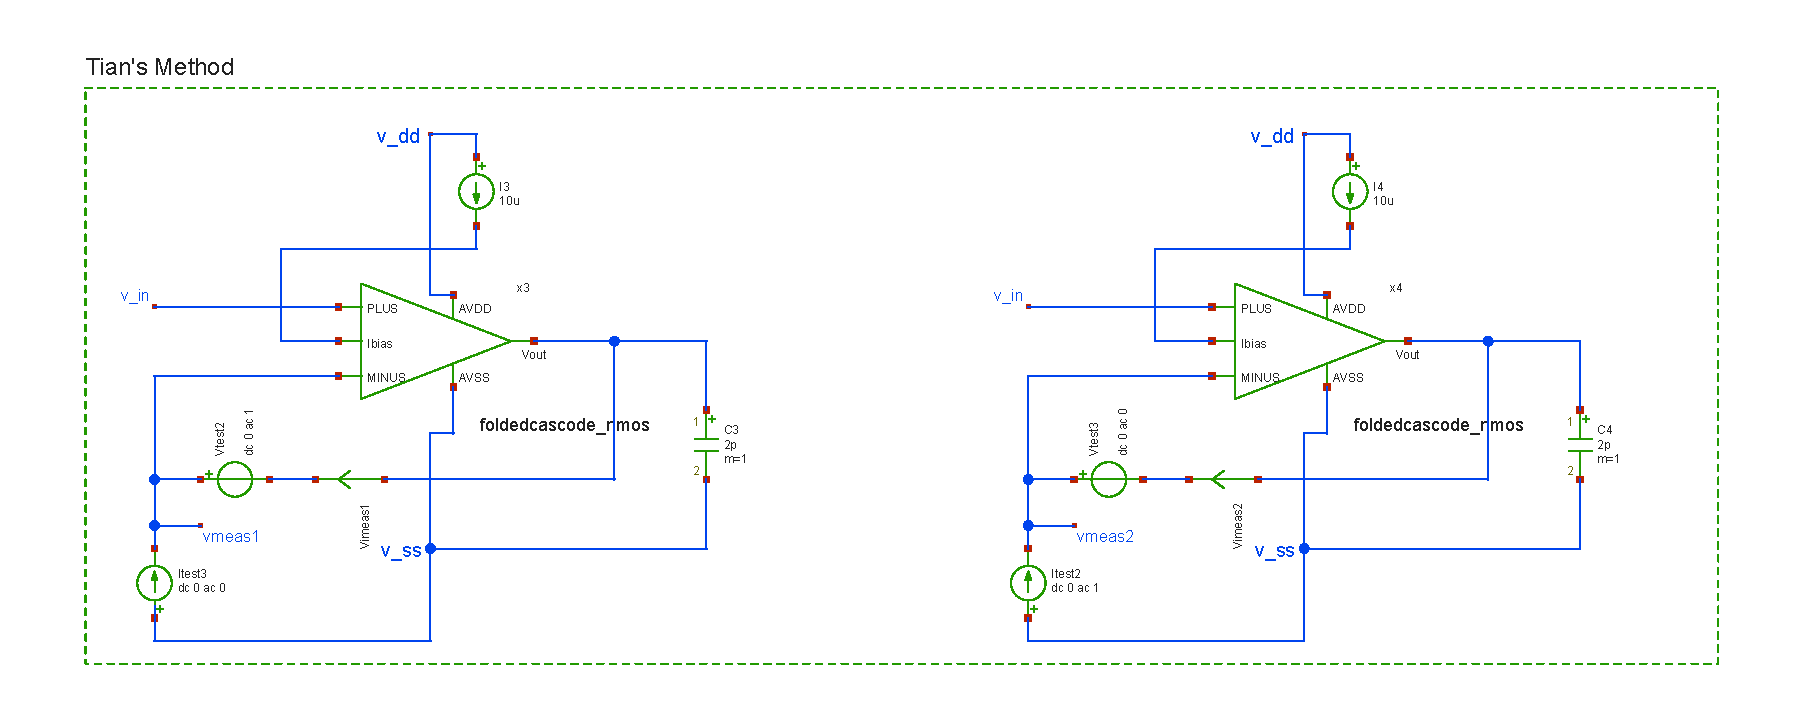
\includegraphics[keepaspectratio]{content/../figures/_fig_loopgain_tian.pdf}}

}

\caption{\label{fig-loopgain-xschem-tian}Loop Gain Setup Tian}

\end{figure}%

\begin{figure}[H]

\centering{

\pandocbounded{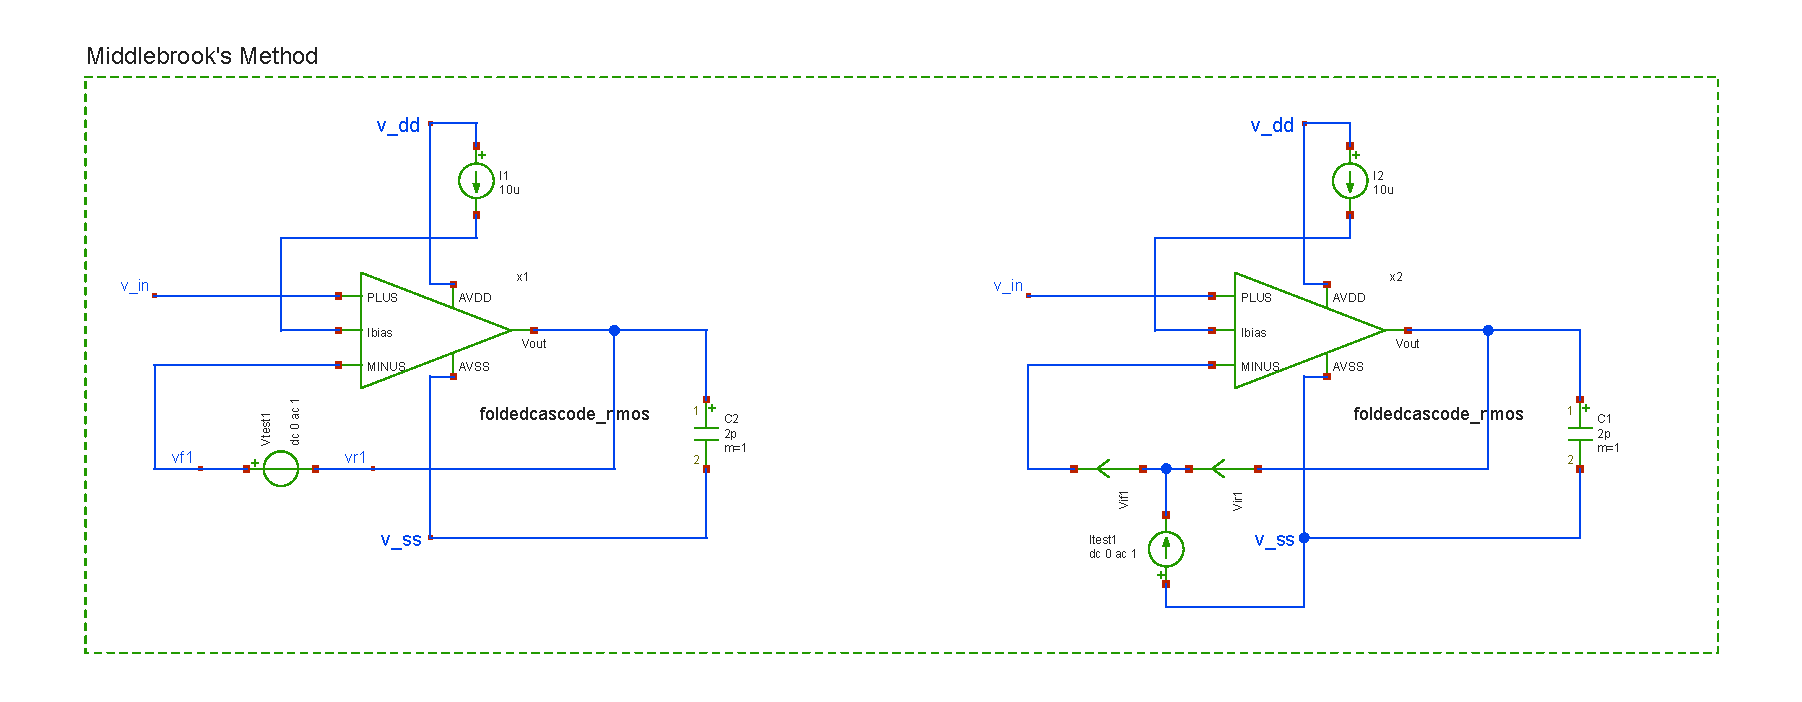
\includegraphics[keepaspectratio]{content/../figures/_fig_loopgain_mb.pdf}}

}

\caption{\label{fig-loopgain-xschem-mb}Loop Gain Setup MiddleBrook}

\end{figure}%

The testbench setup with ngspice code is included in the
schematic\newline
\texttt{./Designs/otas/1\_schematics/tb\_foldedcascode\_nmos\_loopgain.sch}

The loop gain analysis yeilds the following plots which clarifies that
our specifications such as gain and phase margin are met successfully.
See Figure~\ref{fig-loopgain-magnitude} and
Figure~\ref{fig-loopgain-phase} The plots include both Middlebrook's and
Tian's method for loop gain.

\begin{figure}[H]

\centering{

\includegraphics[width=0.8\linewidth,height=\textheight,keepaspectratio]{index_files/mediabag/content/../figures/_fig_loopgain_magnitude.pdf}

}

\caption{\label{fig-loopgain-magnitude}Magnitude middlebrook vs Tian.}

\end{figure}%

\begin{figure}[H]

\centering{

\includegraphics[width=0.8\linewidth,height=\textheight,keepaspectratio]{index_files/mediabag/content/../figures/_fig_loopgain_phase.pdf}

}

\caption{\label{fig-loopgain-phase}Phase middlebrook vs Tian.}

\end{figure}%

\chapter{Corner Simulations for PVT and
Monte-Carlo}\label{corner-simulations-for-pvt-and-monte-carlo}

As already discussed in Section~\ref{sec-ota-simulation}, running every
simulation manually is inefficient and time-consuming.\\
To properly evaluate the OTA, the design must be verified across a wide
range of conditions that influence device behavior.\\
These conditions include:

\begin{enumerate}
\def\labelenumi{\arabic{enumi}.}
\item
  \textbf{Supply voltage variations:}\\
  Practical power supplies do not maintain a fixed nominal value. The
  amplifier therefore needs to be tested across the expected voltage
  tolerance range.{[}3{]}
\item
  \textbf{Temperature variations:}\\
  Analog circuits experience significant parameter shifts across
  temperature. The OTA's performance must therefore be checked over its
  full operating temperature range.{[}3{]}
\item
  \textbf{Process variations:}\\
  Due to unavoidable deviations during wafer fabrication, transistor
  parameters never perfectly match their ideal values.\\
  Foundries provide \emph{corner model files} to represent these
  extremes.\\
  Since NMOS and PMOS devices vary independently, the typical CMOS
  process corners are:\\
  \textbf{SS, SF, TT, FS, and FF}.\\
  All simulations performed so far used only the \textbf{TT}
  corner.{[}3{]}
\end{enumerate}

Together, these variations form the well-known \textbf{PVT
(Process--Voltage--Temperature)} space.\\
A complete design verification requires ensuring that the OTA meets
specifications across \emph{all relevant combinations} of PVT conditions
and input scenarios.\\
This quickly leads to a large number of simulations, each of which must
be evaluated for pass/fail behavior.

To handle this efficiently, two practical strategies exist:

\begin{enumerate}
\def\labelenumi{\arabic{enumi}.}
\item
  \textbf{Experience-based reduction:}\\
  A skilled analog designer can often predict which PVT combinations are
  most critical using analytical intuition.\\
  This allows the number of simulations to be reduced without
  compromising coverage.{[}3{]}
\item
  \textbf{Automated simulation runners:}\\
  Frameworks known as \emph{simulation runners} automate PVT
  exploration. They can execute large batches of simulations, check
  performance against specification limits, and summarize the
  results.{[}3{]}
\end{enumerate}

For this project, we use the open-source simulation runner
\textbf{CACE}.\\
CACE is Python-based and uses a YAML ``datasheet'' that defines:

\begin{itemize}
\tightlist
\item
  the operating conditions,\\
\item
  all required analyses, and\\
\item
  performance metrics with their limits.
\end{itemize}

CACE then automatically generates the required testbenches, runs all
simulations in parallel, extracts results, and compiles them into
documentation.{[}3{]}

A complete CACE setup exists for our OTA.\\
The datasheet file (\texttt{../cace/foldedcascode\_nmos.yaml}) defines
the simulation environment, while the corresponding testbench templates
are:

\begin{itemize}
\tightlist
\item
  AC analysis: \texttt{../cace/templates/foldedcascode-nmos-ac.sch}
\item
  Noise analysis:
  \texttt{../cace/templates/foldedcascode-nmos-noise.sch}
\item
  Transient analysis:
  \texttt{../cace/templates/foldedcascode-nmos-tran.sch}
\end{itemize}

After a successful run, CACE automatically generates a detailed summary
of all results.\\
A portion of this summary is included below:

\begin{tcolorbox}[enhanced jigsaw, titlerule=0mm, bottomrule=.15mm, arc=.35mm, opacitybacktitle=0.6, colbacktitle=quarto-callout-note-color!10!white, title=\textcolor{quarto-callout-note-color}{\faInfo}\hspace{0.5em}{CACE Summary for OTA}, coltitle=black, opacityback=0, leftrule=.75mm, left=2mm, colback=white, toptitle=1mm, breakable, bottomtitle=1mm, colframe=quarto-callout-note-color-frame, rightrule=.15mm, toprule=.15mm]

\emph{netlist source}: schematic

\begin{longtable}[]{@{}
  >{\raggedright\arraybackslash}p{(\linewidth - 18\tabcolsep) * \real{0.1971}}
  >{\raggedright\arraybackslash}p{(\linewidth - 18\tabcolsep) * \real{0.0657}}
  >{\raggedright\arraybackslash}p{(\linewidth - 18\tabcolsep) * \real{0.0657}}
  >{\raggedleft\arraybackslash}p{(\linewidth - 18\tabcolsep) * \real{0.0803}}
  >{\raggedleft\arraybackslash}p{(\linewidth - 18\tabcolsep) * \real{0.1168}}
  >{\raggedleft\arraybackslash}p{(\linewidth - 18\tabcolsep) * \real{0.0876}}
  >{\raggedleft\arraybackslash}p{(\linewidth - 18\tabcolsep) * \real{0.1168}}
  >{\raggedleft\arraybackslash}p{(\linewidth - 18\tabcolsep) * \real{0.0803}}
  >{\raggedleft\arraybackslash}p{(\linewidth - 18\tabcolsep) * \real{0.1241}}
  >{\centering\arraybackslash}p{(\linewidth - 18\tabcolsep) * \real{0.0657}}@{}}
\toprule\noalign{}
\begin{minipage}[b]{\linewidth}\raggedright
Parameter
\end{minipage} & \begin{minipage}[b]{\linewidth}\raggedright
Tool
\end{minipage} & \begin{minipage}[b]{\linewidth}\raggedright
Result
\end{minipage} & \begin{minipage}[b]{\linewidth}\raggedleft
Min Limit
\end{minipage} & \begin{minipage}[b]{\linewidth}\raggedleft
Min Value
\end{minipage} & \begin{minipage}[b]{\linewidth}\raggedleft
Typ Target
\end{minipage} & \begin{minipage}[b]{\linewidth}\raggedleft
Typ Value
\end{minipage} & \begin{minipage}[b]{\linewidth}\raggedleft
Max Limit
\end{minipage} & \begin{minipage}[b]{\linewidth}\raggedleft
Max Value
\end{minipage} & \begin{minipage}[b]{\linewidth}\centering
Status
\end{minipage} \\
\midrule\noalign{}
\endhead
\bottomrule\noalign{}
\endlastfoot
Output voltage ratio & ngspice & gain & 0.98 V/V & 0.996 V/V & any &
0.999 V/V & 1.1 V/V & 1.000 V/V & Pass \\
Bandwidth & ngspice & bw & 1e6 Hz & 5118320.000 Hz & any & 7827360.000
Hz & any & 13271000.000 Hz & Pass \\
Output voltage ratio (MC) & ngspice & gain\_mc & any & 0.671 V/V & any &
0.996 V/V & any & 1.502 V/V & Pass \\
Bandwidth (MC) & ngspice & bw\_mc & 1e6 Hz & 1024950.000 Hz & any &
7454465.000 Hz & any & 91913200.000 Hz & Pass \\
Output noise & ngspice & noise & any & 0.069 mV & any & 0.101 mV & 0.2
mV & 0.134 mV & Pass \\
Settling time & ngspice & tsettle & any & 0.259 us & any & 0.287 us &
1.5 us & 0.320 us & Pass \\
\end{longtable}

\end{tcolorbox}

CACE also produces Python-based plots for each PVT corner and
Monte-Carlo run.\\
The full set of generated plots for our OTA is available in the
repository:\\
\texttt{../cace/\_docs/foldedcascode\_nmos\_1/foldedcascode\_nmos/schematic}

As an example, the figure below shows the \textbf{Noise vs.~Corner}
plot:

\begin{figure}[H]

{\centering \pandocbounded{\includegraphics[keepaspectratio]{content/../figures/_fig_noise_vs_corner.png}}

}

\caption{noise\_vs\_corner}

\end{figure}%

The results of these analyses can be compared to the required
voltage-buffer specifications listed in
Table~\ref{tbl-voltage-buffer-spec}.

\begin{longtable}[]{@{}lcc@{}}
\caption{Voltage buffer
specification}\label{tbl-voltage-buffer-spec}\tabularnewline
\toprule\noalign{}
Specification & OTA & Unit \\
\midrule\noalign{}
\endfirsthead
\toprule\noalign{}
Specification & OTA & Unit \\
\midrule\noalign{}
\endhead
\bottomrule\noalign{}
\endlastfoot
Output voltage error & \(<1\) & \% \\
Total output noise (rms) & \(<0.15\) & mV\textsubscript{rms} \\
Supply current (as low as possible) & \(<14\) & µA \\
Turn-on time & \(<0.4\) & µs \\
Externally provided bias current (nominal) & \(14\) & µA \\
\end{longtable}

\part{Physical Design}

\chapter{Introduction to Layout}\label{introduction-to-layout}

Once, schematic in \textbf{Xschem} is finished, what we have is only the
functional intent of the circuit. At this stage the devices are ideal:
transistors have exactly the width and length we assign, wires have zero
resistance, and parasitics like source/drain capacitances or coupling
between metals are invisible. The layout stage is where this abstraction
becomes \textbf{real silicon geometry}. Here, every transistor must be
drawn in the technology's layers, with actual fingers, source/drain
contacts, guard rings and no component is ideal anymore.

For analog circuits, this step is critical. Small layout choices for
example, placing two input devices slightly asymmetrically, or routing
one input longer than the other can directly show up as offset voltage
or degraded common-mode rejection. In digital design, such effects are
often absorbed by logic thresholds, but in analog design they decide
whether the OTA meets its simulated gain or not.

In other words, schematic defines \emph{``what we want''}, layout
decides \emph{``what we actually get''}. This chapter focuses on showing
how a \emph{folded-cascode OTA} in \textbf{IHP-SG13G2} was translated
from a verified schematic into a manufacturable layout that still
respects matching, symmetry, and parasitic limits.

\section{Layout Toolchain: KLayout}\label{layout-toolchain-klayout}

For the layout implementation, we relied on \emph{KLayout}. It is a
free, scriptable editor that is already integrated with the
\textbf{IHP-SG13G2 open-source PDK} and provided in the \textbf{IIC-OSIC
toolchain}. This makes it possible to perform layout tasks without the
need for commercial software.

All necessary files such as \textbf{Design Rule Checks (DRC)},
\textbf{LVS comparison setups}, and \textbf{Parameterized cells
(PCells)} are directly accessible and supported within KLayout. This
allows devices to be generated, verified, and extracted in a
reproducible way.

For further details, see the \href{https://www.klayout.de/}{KLayout
website}.

\begin{tcolorbox}[enhanced jigsaw, titlerule=0mm, bottomrule=.15mm, arc=.35mm, opacitybacktitle=0.6, colbacktitle=quarto-callout-note-color!10!white, title=\textcolor{quarto-callout-note-color}{\faInfo}\hspace{0.5em}{Using KLayout: Docker vs.~Source Build}, coltitle=black, opacityback=0, leftrule=.75mm, left=2mm, colback=white, toptitle=1mm, breakable, bottomtitle=1mm, colframe=quarto-callout-note-color-frame, rightrule=.15mm, toprule=.15mm]

Our layout work was carried out using \textbf{KLayout v0.30.1}, provided
within the \textbf{IIC-OSIC Docker image}. Since this image is a
prebuilt package, some advanced KLayout or Qt features may not function
as expected.

If KLayout is build from source on your system, most of these
limitations disappear, but in that case \textbf{IHP-SG13G2 technology
files and libraries} must be manually integrated the into your local
setup.

For guidance on this process, a useful resource is this
\href{https://www.youtube.com/watch?v=CSZm3q4rUBg&list=LL&index=24&t=1181s}{Efabless
tutorial (second section by Thomas Perry)}.

\end{tcolorbox}

\chapter{Device-Level Layout
Concepts}\label{device-level-layout-concepts}

Integrated circuit layout translates the schematic into \textbf{physical
layers} on silicon.\\
The IHP-SG13G2 process provides numerous layers such as active/diffusion
regions, poly gates, contacts, multiple metal levels, and passivation.
{[}4{]}\\
Each of these layers plays a role in forming MOSFETs, capacitors,
resistors, and interconnects, further layer specific description for the
IHP PDK can be found on Layout Rules {[}4{]}.

Unlike digital design, where the goal is mainly connectivity, analog
layout must ensure \textbf{matching, symmetry, and parasitic control}.
This is particularly critical in our \textbf{folded-cascode OTA}, where
the differential input pair, current mirrors, and cascode devices
dominate the overall gain, offset, and common-mode rejection ratio
(CMRR). {[}5{]}, {[}6{]}

The following subsections describe the major device-level layout
techniques used in this work, with examples and figures suggested for
illustration.

\section{Matching \& Symmetry}\label{matching-symmetry}

In real silicon, device characteristics are never perfectly uniform
across the die.\\
\textbf{Process gradients} arise during fabrication due to variations in
temperature, pressure, and material distribution. These gradients can be
visualized using concepts similar to \textbf{isobars} (lines with
constant mechanical pressure) or \textbf{isotherms} (lines with same
temperature), where physical properties gradually shift across the wafer
surface {[}6{]}.

Such gradients directly affect threshold voltage, mobility, and oxide
thickness. As a result, two transistors with identical schematic
dimensions may behave differently if placed at different positions on
the chip. For analog circuits like OTAs, these mismatches degrade input
offset, gain, and common-mode rejection ratio (CMRR). In
Figure~\ref{fig-isotherm}, adapted from {[}6{]} thermal gradients caused
by non-uniform heat distributtion across the chip area. Best practice is
to place the devices along the same isotherm.

\begin{figure}[H]

\centering{

\pandocbounded{\includegraphics[keepaspectratio]{index_files/mediabag/content/../figures/_fig_isotherm.pdf}}

}

\caption{\label{fig-isotherm}}

\end{figure}%

\begin{figure}[H]

\centering{

\pandocbounded{\includegraphics[keepaspectratio]{index_files/mediabag/content/../figures/_fig_isobar.pdf}}

}

\caption{\label{fig-isobar}Contradictory to above gradient in mechnical
stress high gradient area should be avoided such as corners and devices
should be placed closer to chip center lines (adapted from {[}6{]}).}

\end{figure}%

To minimize this, layout must enforce \textbf{symmetry}:

\begin{itemize}
\item
  \textbf{Symmetry around an axis.}\\
  Devices intended to operate as pairs, such as the OTA differential
  input transistors, are placed symmetrically about a central axis. This
  ensures that any linear process gradient affects both devices equally,
  preserving balance in their electrical behavior.
\item
  \textbf{Symmetry in current flow.}\\
  Symmetry is not only geometrical but also electrical. The orientation
  of source, drain, and gate terminals is arranged so that current flows
  through matched devices in identical directions. This prevents
  systematic mismatches introduced by unequal diffusion edge proximity
  or channel orientation.
\end{itemize}

Together, these forms of symmetry improve \textbf{matching} the ability
of two devices to exhibit nearly identical electrical performance.
Accurate matching is critical in the OTA's input stage, where small
imbalances directly appear as input offset voltages.

Finally, symmetry must extend to the \textbf{routing}. Interconnect
lengths, widths, and via stacks must be balanced on both sides of the
differential pair. Even with well-matched devices, asymmetric wiring can
introduce additional resistance and capacitance, which shows up as
systematic offset or degraded bandwidth {[}5{]}, {[}6{]}.\\
In our OTA layout, routing symmetry was not only maintained in terms of
path length and via balance, but also extended to the \textbf{choice of
metal layers}. Long interconnects were assigned to \textbf{higher metal
layers} with lower sheet resistance, while short local connections
remained on \textbf{lower metals} for compact access.\\
This combination of length balancing, via symmetry, and layer assignment
ensured that both differential branches exhibited comparable parasitic
resistance and capacitance, preserving matching despite unavoidable
topological constraints.

\section{Multi-Fingering}\label{multi-fingering}

When MOSFETs are designed with very wide channel widths, implementing
them as a single continuous device introduces several problems. A long,
uninterrupted polysilicon gate line introduces significant
\textbf{polysilicon gate resistance}, which degrades high-frequency
behavior and increases phase delay. At the same time, the enlarged
diffusion regions lead to higher source and drain junction capacitances,
creating substantial loading on sensitive circuit nodes. Finally, wide
monolithic devices suffer in terms of matching: process gradients across
the active area are no longer averaged, making these devices more
vulnerable to systematic variation and random mismatch effects {[}5{]},
{[}6{]}.

The solution is \textbf{multi-fingering}: dividing the wide transistor
into several narrower, identical fingers that are connected in parallel.
This segmentation reduces gate resistance (shorter poly stripes),
distributes junction capacitances more evenly, and improves statistical
matching by averaging across multiple smaller units.

In our OTA, the \textbf{tail current source} required a total width of
8.5 µm. Instead of realizing it as a single device, it was split into
\textbf{four fingers of 2.125 µm each}. This segmentation reduced the
distributed gate resistance, improved current uniformity, and made gate
routing more compact and symmetrical, while maintaining acceptable
junction capacitance at the high-impedance tail node. Similarly,
majority of transistors were implemented in multi-finger form to balance
parasitic capacitances and maintain symmetry across branches.

\begin{figure}[H]

\centering{

\pandocbounded{\includegraphics[keepaspectratio]{content/../figures/_fig_tail_transistor.png}}

}

\caption{\label{fig-ota_tail}Represents the tail transistor in our
layout with 4 fingers instead of one huge block lead to well matched
layout with other transistors and clean routing.}

\end{figure}%

Despite its benefits, multi-fingering comes with trade-offs:\\
- \textbf{Increased routing overhead}, since all fingers must be tied
together with well-balanced interconnect.\\
- \textbf{Extra junction perimeters}, which can increase total parasitic
capacitance if the layout is not compacted carefully.\\
- \textbf{Via placement sensitivity}, as each finger requires
source/drain contacts and vias; poor via distribution can lead to
resistance mismatches or electromigration concerns. Using 2 vias is
always recommended.{[}6{]}

For this reason, multi-fingering is often combined with other layout
strategies.\\
\textbf{Dummies} are placed at the array edges to shield active fingers,
while \textbf{common-centroid arrangements} may be used for further
gradient cancellation. This combined approach was applied in our OTA's
diffpair, ensuring both parasitic reduction and high matching fidelity.

\begin{tcolorbox}[enhanced jigsaw, titlerule=0mm, bottomrule=.15mm, arc=.35mm, opacitybacktitle=0.6, colbacktitle=quarto-callout-note-color!10!white, title=\textcolor{quarto-callout-note-color}{\faInfo}\hspace{0.5em}{How to calculate minimum number of fingers}, coltitle=black, opacityback=0, leftrule=.75mm, left=2mm, colback=white, toptitle=1mm, breakable, bottomtitle=1mm, colframe=quarto-callout-note-color-frame, rightrule=.15mm, toprule=.15mm]

Determining the appropriate number of fingers for a wide MOSFET is not
arbitrary; it requires balancing several parasitic and physical effects.

As excessive fingering increases total diffusion perimeter and further
elevating the total source/drain junction capacitance.

Therefore, selecting the \emph{minimum} number of fingers that satisfies
these electrical and physical constraints is essential for achieving
optimal analog performance.

A rigorous methodology for estimating this minimum finger count
considering gate resistance limits, diffusion capacitance contributions,
layout symmetry, and manufacturability is presented in \textbf{Section
7.6: Finger Count Estimation}, where all the equations and procedures
are discussed in detail.

\end{tcolorbox}

\section{Dummy Devices}\label{dummy-devices}

Even when multi-fingering is used, the \textbf{edge fingers} of a device
array experience different fabrication conditions compared to the inner
fingers. At the boundary between active diffusion and isolation (STI),
variations in oxide growth, stress, and implant profiles create
\textbf{edge effects} that change threshold voltage, carrier mobility,
and junction capacitance {[}5{]}.\\
If left unaddressed, these systematic differences degrade device
matching, particularly in sensitive analog structures such as the OTA
input pair or current mirrors.

To eliminate this, \textbf{dummy devices} are placed at the ends of
transistor arrays. They act as sacrificial neighbors, ensuring that all
\emph{active} devices are surrounded by identical environments.\\
This makes the inner devices more uniform, effectively shielding them
from edge-related mismatches.{[}6{]}

Connection of dummy devices can vary across design flows:\\
- In some methodologies, dummy gates are left \textbf{floating}, since
their only role is geometric.\\
- In others, dummies are \textbf{tied to supply rails} (AVDD or AVSS) to
avoid LVS errors and ensure consistent recognition by verification
tools.

In our OTA, Dummy devices were placed at the edges of all the MOSFET's.
This ensured that all transistors within the OTA operated in
well-matched environments, minimizing systematic offset.

\begin{tcolorbox}[enhanced jigsaw, titlerule=0mm, bottomrule=.15mm, arc=.35mm, opacitybacktitle=0.6, colbacktitle=quarto-callout-important-color!10!white, title=\textcolor{quarto-callout-important-color}{\faExclamation}\hspace{0.5em}{Important Implementation Note}, coltitle=black, opacityback=0, leftrule=.75mm, left=2mm, colback=white, toptitle=1mm, breakable, bottomtitle=1mm, colframe=quarto-callout-important-color-frame, rightrule=.15mm, toprule=.15mm]

In our OTA layout, dummy devices were implemented as \textbf{complete
MOSFETs} with their gates explicitly tied to \textbf{AVDD} or
\textbf{AVSS}.\\
This was necessary because in \textbf{KLayout}, adding an extra finger
with an unconnected gate/source/drain is not recognized as a dummy. LVS
then fails due to netlist mismatches.

To ensure \textbf{LVS clean results}, we:\\
- Added dummy devices explicitly in the schematic.\\
- Connected all terminals to valid nets.\\
- Replicated the same connections in layout.

\end{tcolorbox}

\section{Interdigitated Layout}\label{interdigitated-layout}

When two matched transistors are placed adjacent to each other but in
separate diffusion regions, each device is exposed to a slightly
different portion of the process gradient across the chip. As a result,
parameters such as threshold voltage, carrier mobility, and oxide
thickness vary between them, leading to a systematic mismatch even
though both devices have identical drawn dimensions.

The \textbf{interdigitated layout technique} addresses this issue by
physically alternating the unit devices of a matched pair or array.
Instead of grouping devices as AABB, the transistors are arranged in an
alternating or mirrored pattern such as \textbf{ABAB} or \textbf{ABBA},
where \emph{A} and \emph{B} represent identical unit devices belonging
to two matched elements.\\
Through this alternating placement, each device is spatially distributed
across the gradient, allowing it to experience regions of both higher
and lower process variations. As a result, the local fabrication
differences are \textbf{averaged} out across all unit fingers, and the
two devices become physically and electrically better matched under real
process conditions.

\begin{figure}[H]

\centering{

\pandocbounded{\includegraphics[keepaspectratio]{index_files/mediabag/content/../figures/_fig_abba.pdf}}

}

\caption{\label{fig-abba}Shows the interdigitated layout pattern
``ABBA'' (right) of current mirror schematic of NMOS-FETs with current
ratio 1:1(left). The ``D'' gates in layout represent the Dummy
transistors.{[}6{]}}

\end{figure}%

This concept can be visualized by imagining a linear gradient across the
x-axis of the die. If one device occupies the left region and the other
the right, they sample distinct gradient values. However, when their
unit fingers are interleaved, each device occupies multiple local
regions along the gradient, resulting in matched \emph{average
parameters}.

In practice, interdigitation is most effective for \textbf{linear
process gradients} along one direction and is often used for
\textbf{matched transistor pairs, current mirrors, or differential input
stages}.\\
For two-dimensional gradients or more complex variations, this technique
is typically extended using \textbf{common-centroid placement}
(discussed in the next section).

In the folded cascode OTA, \textbf{interdigitation} was applied to the
active loads and bias current mirrors. This layout ensured that each
mirrored transistor experienced an equivalent average doping and oxide
thickness, resulting in better current matching, symmetrical output
swing, and reduced systematic offset in bias generation.

\section{Common-Centroid Layout}\label{common-centroid-layout}

While interdigitation cancels \textbf{first-order linear gradients}
along a single direction, it cannot fully correct for
\textbf{two-dimensional or higher-order variations} such as diagonal
gradients or wafer-level curvature. For more advanced matching
requirements such as in precision current mirrors or differential pairs
in high-gain OTAs \textbf{common-centroid layout} is used.

In a common-centroid configuration, matched devices are arranged so that
their geometric centers, or \textbf{centroids}, coincide. Each device is
distributed symmetrically around a central point such that any gradient
whether horizontal, vertical, or diagonal affects both devices equally
when averaged over their area. This approach effectively cancels
first-order gradient components in both axes and reduces second-order
effects as well {[}6{]}.

Conceptually, the centroid layout extends the interdigitated approach
into two dimensions. For example, four identical transistors can be
arranged symmetrically around a central point in an AB/BA pattern,
forming what is effectively a square or cross-shaped configuration.

\begin{figure}[H]

\centering{

\pandocbounded{\includegraphics[keepaspectratio]{index_files/mediabag/content/../figures/_fig_common_centroid.pdf}}

}

\caption{\label{fig-common_centroid.figure}Illustrates how common
centroid configuration can be achieved (right) of current mirror
schematic of NMOS-FETs with current ratio 1:1(left). Its clear that
devices are extremely symmetrical along X-and Y-axis, however routing
always introduces some asymmetry which can be neglected for time being.
Here, space is intentionally left between transistors for clear visuals
and understanding. The ``D'' gates in layout represent the Dummy
transistors.}

\end{figure}%

Although each individual finger occupies a slightly different position
on the chip and therefore a slightly different local environment the
geometric center (centroid) of all devices coincides. This ensures that
the averaged electrical properties of each device are identical,
effectively cancelling first-order process gradients across both axes.

In our folded-cascode OTA, the \textbf{diff pair} was laid out using a
\textbf{common-centroid pattern} derived from the AB/BA principle. This
was essential to maintain current accuracy and minimize systematic gain
variation.\\
The layout ensured that matched transistors experienced a balanced
environment, even in the presence of lateral thermal gradients or stress
gradients from nearby metal density variations.

\textbf{Routing Considerations:}\\
Achieving symmetry in interconnect is as critical as maintaining
symmetry in device placement. In principle, identical path lengths,
matched metal layers, and mirrored via distributions help ensure that
the parasitic resistances and capacitances experienced by paired devices
remain equal. However, practical experience reveals that \emph{strict
geometric symmetry does not always translate into optimal electrical
symmetry}, especially in multi-metal processes such as IHP-SG13G2.

A notable observation from our layout work illustrates this point
clearly. In most of tech nodes including IHP-sg13g2 lower metal layers
(Metal1, Metal2) exhibit \textbf{higher sheet resistance}, they are
typically used for short internal routing, while upper metals provide
lower resistance and reduced coupling.\\
In an attempt to maximize matching, the initial differential-pair
routing was implemented almost entirely on the lowest metal layers
(Metal1 and Metal2), with perfectly mirrored path lengths and identical
layer usage on both branches. Although geometrically symmetric, this
approach resulted in \textbf{severe performance degradation}: the
differential pair failed to operate correctly.\\
Post-layout analysis revealed that the close proximity of long parallel
segments on the same or adjacent lower metal layers introduced
\textbf{excessive lateral and broadside capacitances}, overwhelming the
high-impedance input nodes and collapsing the expected differential
behavior.

This led to a revised routing strategy grounded in parasitic-aware
symmetry rather than purely geometric symmetry. The final solution
employed a combination of \textbf{Metal1, Metal2, and Metal3}, arranged
such that the two branches remained electrically matched but \textbf{did
not rely on identical metal layers running in close parallel}. Where
parallelism was unavoidable, routing was staggered (e.g., \(Metal_n\)
with \(Metal_{n+2}\)) to reduce capacitive coupling.\\
This parasitic-conscious routing produced a substantial improvement in
OTA performance, restoring gain and achieving stable differential
operation.

\begin{figure}[H]

\centering{

\pandocbounded{\includegraphics[keepaspectratio]{index_files/mediabag/content/../figures/_fig_diffpair.pdf}}

}

\caption{\label{fig-diff_pair.figure}Modified Layout of OTA's
Differential Pair with labelled terminals. All used layers are described
in bottom-right corner. The box around the pair is called Guard Ring
which is tied to VSS, also acts as body terminal for all the devices and
is explained in Chapter - \emph{Parasitics and Prevention}.}

\end{figure}%

These findings highlight that in precision analog layout,
\textbf{symmetry must be interpreted electrically, not only
geometrically}. Effective matching requires an awareness of
sheet-resistance gradients, metal-layer coupling, and the spatial
distribution of parasitics.

Meticulous routing decisions layer staggering, spacing, orthogonality,
and controlled via placement often determine whether a differential
structure performs ideally or fails entirely.

\section{Finger Count Estimation (Minimum Number of
Fingers)}\label{finger-count-estimation-minimum-number-of-fingers}

This section establishes a systematic method for estimating the
\textbf{minimum number of fingers} \(N_f\) required for a wide MOSFET
such that\\
(i) the \textbf{distributed gate resistance} remains below acceptable
limits, and\\
(ii) the \textbf{junction capacitances} introduced by segmentation do
not dominate the node dynamics.\\
The methodology follows the classical treatment of \textbf{gate
resistance}, \textbf{thermal/gate noise}, and \textbf{diffusion
capacitance scaling} described in {[}7{]}, {[}8{]}.

For a device with total drawn width \(W_{tot}\) and channel length
\emph{L}, splitting the device into \(N_f\) identical fingers results in
an effective per-finger width

\[
W_f = \frac{W_{\text{tot}}}{N_f}.
\]

Selecting \(N_f\) is therefore an exercise in determining how narrow
each finger can be made before device performance becomes degraded by
source drain capacitance, or minimum-geometry constraints.

The following design principles guide the estimation procedure:

\subsection{Gate Resistance Requirement (Low-Noise
Criterion)}\label{gate-resistance-requirement-low-noise-criterion}

As a practical thumb rule used in low-noise analog design:

\begin{quote}
Each finger width \(W_f\) must be chosen such that the \textbf{gate
resistance} of that finger is \textbf{less than} the inverse
transconductance \(1/g_m\) associated with that finger.\\
For high-performance or low-noise applications, the gate resistance
should preferably be in the range of\\
\[
R_g < \frac{1}{5 g_m} \quad \text{to} \quad R_g < \frac{1}{10 g_m}
\]
\end{quote}

This condition ensures that the \textbf{gate thermal noise contribution}
remains significantly below the \textbf{channel thermal noise},
preventing degradation of input-referred noise or gain.{[}8{]}

Basically, we compare the \textbf{channel thermal noise} with the
\textbf{gate-resistance thermal noise}, and we solve to get the value of
\(N_f\) ensuring that gate noise remains well below channel noise.

\textbf{Channel noise:}

\[
\overline{v_{n,\text{ch}}^2} = \frac{4 k T\, \gamma}{g_m}
\]

\textbf{Gate-resistance noise:}

\[
\overline{v_{n,\text{g}}^2} = \frac{4 k T R_{sheet} W}{3 L N_f^2} 
\]

where,

\begin{itemize}
\tightlist
\item
  \emph{k} is Boltzmann's constant,
\item
  \emph{T} is the absolute temperature,
\item
  \(\gamma\) is the noise factor
\item
  \(g_m\), W \& L are the transconductance, width and length of the
  device.
\end{itemize}

In our application, Channel noise is 5 times that of Gate-resistance
noise.

\subsection{Noise Model Adjustment Based on Channel
Length}\label{noise-model-adjustment-based-on-channel-length}

The optimization also depends on the \textbf{noise coefficient
\emph{\(\gamma\)}} in the MOSFET thermal noise model. The correct value
of \(\gamma\) depends on the channel length:

\begin{itemize}
\tightlist
\item
  If \(L < 3 \times L_{min}\), then \(\gamma = 1\)\\
\item
  otherwise, \(\gamma = \frac{2}{3}\)
\end{itemize}

Because shorter-channel devices exhibit stronger velocity saturation and
increased thermal noise.

\subsection{Minimum Geometry
Constraint}\label{minimum-geometry-constraint}

The number of fingers must also satisfy:

\[
\frac{W_{\text{tot}}}{N_f} > L_{\min},
\]

because excessively narrow fingers approach the \textbf{minimum
manufacturable width} and exhibit strong proximity effects, increased
mismatch, and higher perimeter capacitance.{[}7{]} For the IHP-SG13G2
130-nm process used here, as the name suggests the minimum channel
length is:

\[
L_{\min} = 0.13\,\mu\text{m}.
\]

This constraint prevents unrealistic fingering.

\subsection{Even Number of Fingers (Practical Layout
Consideration)}\label{even-number-of-fingers-practical-layout-consideration}

Although electrically permissible, \textbf{odd-valued finger counts}
typically complicate routing and disrupt symmetry. Although in fewer
cases odd numbered fingers are used as well.\\
But, a practical recommendation particularly in differential or
current-mirror structures is:

Choose the \textbf{minimum even number of fingers} \(N_f\) that
satisfies the electrical and geometrical constraints. Even segmentation
simplifies mirrored routing, centroid or interdigitated arrangements,
and guard ring alignment.

\begin{tcolorbox}[enhanced jigsaw, titlerule=0mm, bottomrule=.15mm, arc=.35mm, opacitybacktitle=0.6, colbacktitle=quarto-callout-note-color!10!white, title=\textcolor{quarto-callout-note-color}{\faInfo}\hspace{0.5em}{Number of fingers Calculation using Python Script}, coltitle=black, opacityback=0, leftrule=.75mm, left=2mm, colback=white, toptitle=1mm, breakable, bottomtitle=1mm, colframe=quarto-callout-note-color-frame, rightrule=.15mm, toprule=.15mm]

To support the design methodology described above, a dedicated
\textbf{Python script} has been developed to automatically compute the
\textbf{minimum number of fingers} required for any given MOSFET
width.\\
The script implements the \textbf{thumb-rule constraints} introduced
above. By providing required parameters, the script outputs the
\textbf{minimum feasible even-valued \(N_f\)} that satisfies all
electrical constraints.

The detailed path for script can be found in \emph{Appendix - C}.

\end{tcolorbox}

\chapter{Design Rule Checking (DRC)}\label{design-rule-checking-drc}

The transition from an electrical schematic to a manufacturable
integrated circuit relies on the integrity of the \textbf{layout}, which
represents the true physical interface between design and fabrication.
While schematic-level verification ensures functional correctness and
circuit performance, it is the layout that determines whether the
circuit can be fabricated reliably within the limits of the chosen
process.\\
To formalize and automate this verification, the semiconductor industry
have \textbf{Design Rule Checking (DRC)} a systematic comparison of the
layout geometry against a set of process-specific constraints provided
by the foundry or technology provider (in our case IHP-PDK Authors).

\section{Fundamentals of DRC}\label{fundamentals-of-drc}

Design Rule Checking is a geometric verification step that ensures a
layout adheres to the \textbf{minimum/maximum feature sizes, spacings,
enclosures, and overlaps} defined by the fabrication process.\\
Each layer in a modern BiCMOS process (e.g.~diffusion, polysilicon,
metal interconnects, and vias) is subject to numerous rules derived from
the physical limitations of photolithography, etching, and deposition
steps.\\
Violating these constraints can lead to a spectrum of manufacturing
defects: short-circuits due to over-etching, open connections caused by
lithographic line thinning, or parametric variations resulting from
disuniform film growth.\\
Thus, DRC forms the \textbf{first line of defense} against
non-manufacturable or yield-critical layouts.

The design rules themselves originate from \textbf{process
specifications}. Foundries experimentally determine the tolerances of
their technology through test structures that measure lithographic
resolution, etch bias, and alignment accuracy between layers. From these
experiments, statistical margins are extracted and translated into
deterministic layout constraints expressed as rules such as
\emph{minimum Active width = 0.15 µm} or \emph{minimum spacing between
Metal1 lines = 0.18 µm}. {[}4{]} As discussed in {[}6{]}, these rules
balance manufacturability with design density: tighter rules enable
compact designs but raise the risk of yield loss, while relaxed rules
increase process robustness at the expense of silicon area.

\section{Technology Dependence and Process
Node}\label{technology-dependence-and-process-node}

Every \textbf{technology node} for instance, 130 nm, 65 nm, or 28 nm
defines its own set of DRC parameters. These parameters evolve with
advances in lithographic precision, material systems, and transistor
architecture. At older nodes such as \textbf{0.35 µm or 0.25 µm}, DRC
rules mainly governed planar dimensions and spacing; however, in sub-100
nm processes, additional considerations such as \textbf{antennas, stress
effects, and metal density gradients} are incorporated. Consequently,
the complexity of DRC rules increases exponentially as the process
geometry scales down.{[}5{]}

The \textbf{Process Design Kit (PDK)} serves as the bridge between the
foundry and the design environment.\\
It encapsulates all technology-specific information design rules, layer
definitions, device models, parasitic extraction parameters, and
layout-Vs-schematic (LVS) configurations into a single framework usable
by EDA tools.\\
The DRC deck, which is a formalized file (often written in languages
such as SVRF or Python-based scripts for tools like KLayout), encodes
these geometric constraints in machine-readable form. When the layout is
processed through the DRC engine, each polygon and layer is
algorithmically compared against the rule database to identify
violations.

In the case of the \textbf{IHP SG13G2 130 nm BiCMOS process}, used
throughout this work, the \emph{IHP-PDK} provides a comprehensive DRC
rule set defining all critical geometrical limits from
diffusion-to-diffusion spacing and via enclosures to hierarchical
density checks of upper metal layers, {[}4{]}. The \emph{IHP-PDK} also
supplies detailed technology definition files that can be manually
integrated into layout tools such as KLayout. However, since the
\emph{IHP-PDK} is part of the \emph{IIC-OSIC} open-source toolchain,
these technology files and rule decks are already pre-configured within
the provided Docker image, offering an optimized and reproducible setup
for DRC verification.

In addition, the PDK documentation includes a complete layer table
defining all process layers, along with descriptions of forbidden layers
reserved for internal fabrication use, grid rules, and the full list of
DRC constraints illustrations. This document has served as the primary
reference for understanding the process and implementing all layout
structures in this work. Hence, even within an open-source environment,
the design remains \textbf{foundry-compliant}, physically realizable,
and fully aligned with the manufacturing specifications of the SG13G2
process.

\section{Importance in the Design
Flow}\label{importance-in-the-design-flow}

DRC plays a pivotal role in ensuring that the \textbf{layout is not only
electrically correct but physically manufacturable}.\\
As mentioned before, an unverified layout might pass all functional and
electrical simulations yet still fail in fabrication because certain
features violate lithographic limits or introduce yield-limiting
defects. Typical examples include insufficient metal spacing leading to
shorts, or inadequate enclosure of contacts resulting in open circuits
after etching.\\
By enforcing DRC compliance before tape-out, the designer ensures that
the design adheres to the \textbf{design-for-manufacturability (DFM)}
principles required for reproducible production.

Furthermore, DRC compliance is not merely a binary condition of ``pass
or fail.'' It also acts as a \textbf{metric of process awareness}: a
DRC-clean layout demonstrates the designer's adherence to technology
constraints and reflects a realistic understanding of fabrication
tolerances. In professional design flows, foundries refuse to fabricate
any layout that fails DRC, as doing so would waste mask costs and
process time.

Therefore, DRC stands as the final checkpoint between design creativity
and physical implementation a gate that ensures the \textbf{logical
intent of the schematic can manifest in silicon without violation of the
underlying physics}.

\section{Practical Implementation of Design Rule
Checking}\label{practical-implementation-of-design-rule-checking}

As discussed in earlier chapters, the \textbf{layout is the sole design
entity that directly communicates with fabrication}. Neither schematic
diagrams nor behavioral models ever reach the foundry only the geometric
database (typically in GDSII or OASIS format) generated from the layout
is delivered for mask generation and processing.\\
In this sense, \textbf{Design Rule Checking (DRC)} serves as the
mechanism through which the \emph{language of design} is translated into
the \emph{language of manufacturing}. It guarantees that every
transistor, interconnect, and via is drawn within the lithographic and
etching tolerances established by the process technology. This alignment
between layout geometry and process capability is essential to achieving
both functional yield and long-term device reliability.\\
To borrow the phrasing of {[}5{]}, \emph{``a perfect schematic means
nothing without a correct layout.''}\\
DRC ensures that this correctness is quantifiable and verifiable it
enforces the discipline that transforms circuit theory into a physically
reproducible artifact, one capable of moving confidently from layout
database to wafer fabrication.

In this work, all DRC verification was performed using \textbf{KLayout}
as part of the \textbf{IIC-OSIC open-source toolchain}, which integrates
the \textbf{IHP SG13G2 130 nm BiCMOS process}. The PDK provides complete
DRC rule decks in the form of Python-based macros that systematically
check every process layer and layer combination diffusion overlaps, via
enclosures, contact spacings, metal width and density requirements, and
top-metal clearance to the passivation opening.

The DRC engine performs a hierarchical scan of the layout, flags any
violations, and displays annotated markers directly within the KLayout
interface for review. Each violation encountered during the layout phase
was analyzed and corrected at either the device or routing level until
the design achieved a fully \textbf{DRC-clean status}. This verified
layout therefore not only satisfies the intended schematic connectivity
but also conforms to every \textbf{physical constraint required for
successful fabrication}. Through this process, DRC validation in KLayout
establishes the final and most critical bridge between the abstract
world of circuit design and the tangible reality of silicon
manufacturing where compliance with foundry rules ensures that what is
drawn can, indeed, be built.

\subsection{Types of DRC Scripts in the IHP SG13G2
Process}\label{types-of-drc-scripts-in-the-ihp-sg13g2-process}

The \textbf{IHP SG13G2 PDK} provides two distinct DRC scripts, each
corresponding to a specific level of design compliance and verification
rigor. These scripts are referred to as \textbf{sg13g2\_minimal} and
\textbf{sg13g2\_maximal} rule decks. Both are written as Python macros
configured within the KLayout environment and can be executed directly
from the \emph{Macros Development} interface.

\begin{enumerate}
\def\labelenumi{\arabic{enumi}.}
\item
  The \textbf{sg13\_g2\_minimal DRC deck} enforces the \emph{standard
  design rules} of the process: These rules define the \textbf{mandatory
  fabrication constraints} that must be satisfied to ensure the layout
  is physically manufacturable. Violations of these checks typically
  indicate errors that could prevent successful chip production or cause
  fatal defects in the fabricated devices. Examples include insufficient
  metal spacing, missing via enclosures, or incorrect layer overlaps.
  List of minimal rules can be found
  \href{https://github.com/IHP-GmbH/IHP-Open-PDK/blob/main/ihp-sg13g2/libs.tech/klayout/tech/drc/README_minimal.md}{here}.
\item
  The \textbf{sg13\_g2\_maximal DRC deck}, in contrast, applies the
  \emph{recommended design rules}: These rules contain both
  \textbf{mandatory fabrication constraints} and \textbf{non-mandatory}
  therefore are intended to improve overall \textbf{manufacturability,
  process reliability, and yield consistency}. They provide design hints
  to minimize parametric variability, such as improving parasitics,
  preventing latch-ups, or avoiding angles that can introduce stress
  points during fabrication. While designs that only pass the minimal
  check are still fabricable, running the sg13\_g2\_maximal script
  ensures the layout adheres to \textbf{best practices} for long-term
  robustness and high-yield performance. List for maximal rules can be
  found
  \href{https://github.com/IHP-GmbH/IHP-Open-PDK/blob/main/ihp-sg13g2/libs.tech/klayout/tech/drc/README_maximal.md}{here}.
\end{enumerate}

\subsection{Performing DRC in KLayout}\label{performing-drc-in-klayout}

As mentioned in the \emph{Known Issues} section, DRC cannot be executed
in KLayout solely by relying on direct tools or commands. Instead, a
specific workflow must be followed. Within the \textbf{Macros
Development} interface of KLayout, there is a dedicated \textbf{DRC
section} that lists all available rule scripts for the selected
technology. To perform DRC, the user must select the desired rule deck
either \emph{sg13\_g2\_minimal} or \emph{sg13\_g2\_maximal} and then
execute the corresponding script.

\begin{figure}[H]

\centering{

\pandocbounded{\includegraphics[keepaspectratio]{index_files/mediabag/content/../figures/_fig_macro_devs.pdf}}

}

\caption{\label{fig-macro-dev}Macro Development interface with DRC
Results in Console}

\end{figure}%

Once the check is complete, the list of errors appears in the
\textbf{output console} below the editor window. Unfortunately, due to
current tool limitations, KLayout does not automatically generate a
separate \textbf{DRC report file}. This means that the error list cannot
be reloaded, filtered, or revisited directly within the tool after the
session ends. Furthermore, some \textbf{Qt-based interactive functions}
(intended to automatically highlight or open error markers) are not
fully supported within the Docker image of the IIC-OSIC toolchain.

To address this limitation, a \textbf{custom Python script} was
developed in this work to automate the error-handling process. The
script parses the raw DRC output copied from the KLayout console and
filters the messages to produce a clean, structured list of all raised
violations that require manual correction. This greatly simplifies the
debugging workflow by identifying unique errors and mapping them to
their respective layer categories.

\subsection{DRC Automation Script}\label{drc-automation-script}

This is the automation script used for processing DRC results:

\begin{tcolorbox}[enhanced jigsaw, titlerule=0mm, bottomrule=.15mm, arc=.35mm, opacitybacktitle=0.6, colbacktitle=quarto-callout-note-color!10!white, title=\textcolor{quarto-callout-note-color}{\faInfo}\hspace{0.5em}{Script}, coltitle=black, opacityback=0, leftrule=.75mm, left=2mm, colback=white, toptitle=1mm, breakable, bottomtitle=1mm, colframe=quarto-callout-note-color-frame, rightrule=.15mm, toprule=.15mm]

DRC Errors Check

This script gives 2 functions: 1st needs the the errors copied from
KLayout to be pasted in drc\_log function inside script and than run the
script. It can be tidious to change script again and again. Therefore,
not recommended.

For 2nd function just run the script and paste your errors copied from
KLayout in the terminal and press enter and DONE. By default, script
uses this function.

\begin{Shaded}
\begin{Highlighting}[]
\CommentTok{\# 2nd Funtion}

\KeywordTok{def}\NormalTok{ parse\_drc\_errors\_new():}
    \BuiltInTok{print}\NormalTok{(}\StringTok{" Paste your DRC error log below. Press Enter twice to finish:"}\NormalTok{)}
    
    \CommentTok{\# Collect multiline input}
\NormalTok{    lines }\OperatorTok{=}\NormalTok{ []}
    \ControlFlowTok{while} \VariableTok{True}\NormalTok{:}
\NormalTok{        line }\OperatorTok{=} \BuiltInTok{input}\NormalTok{()}
        \ControlFlowTok{if}\NormalTok{ line.strip() }\OperatorTok{==} \StringTok{""}\NormalTok{:}
            \ControlFlowTok{break}
\NormalTok{        lines.append(line)}
    
    \BuiltInTok{print}\NormalTok{(}\StringTok{"}\CharTok{\textbackslash{}n}\StringTok{⚠️ Rules with errors :"}\NormalTok{)}
\NormalTok{    i}\OperatorTok{=}\DecValTok{0}
    \ControlFlowTok{for}\NormalTok{ line }\KeywordTok{in}\NormalTok{ lines:}
        \ControlFlowTok{if} \StringTok{"error(s)"} \KeywordTok{in}\NormalTok{ line:}
            \ControlFlowTok{try}\NormalTok{:}
\NormalTok{                rule, error\_text }\OperatorTok{=}\NormalTok{ line.split(}\StringTok{":"}\NormalTok{)}
\NormalTok{                error\_count }\OperatorTok{=} \BuiltInTok{int}\NormalTok{(error\_text.strip().split()[}\DecValTok{0}\NormalTok{])}
                \ControlFlowTok{if}\NormalTok{ error\_count }\OperatorTok{\textgreater{}=} \DecValTok{1}\NormalTok{:}
                    \BuiltInTok{print}\NormalTok{(}\SpecialStringTok{f"}\SpecialCharTok{\{}\NormalTok{rule}\SpecialCharTok{.}\NormalTok{strip()}\SpecialCharTok{\}}\SpecialStringTok{: }\SpecialCharTok{\{}\NormalTok{error\_count}\SpecialCharTok{\}}\SpecialStringTok{ error(s)"}\NormalTok{)}
\NormalTok{                    i}\OperatorTok{=}\DecValTok{1}

            \ControlFlowTok{except} \PreprocessorTok{ValueError}\NormalTok{:}
                \ControlFlowTok{continue}
    
    \ControlFlowTok{if}\NormalTok{ i}\OperatorTok{==}\DecValTok{0}\NormalTok{:}
        \BuiltInTok{print}\NormalTok{(}\StringTok{"Congrats! No error"}\NormalTok{)}
\end{Highlighting}
\end{Shaded}

\begin{Shaded}
\begin{Highlighting}[]
\CommentTok{\# Run the parser}
\NormalTok{parse\_drc\_errors\_new()}
\end{Highlighting}
\end{Shaded}

\end{tcolorbox}

To use the script, simply copy the DRC Errors from console output from
KLayout, paste it into the terminal running the Python program, and the
script will generate a concise summary of the errors that remain to be
corrected manually in the layout. This script could also be found in
\emph{Appendix - C}.

\begin{tcolorbox}[enhanced jigsaw, titlerule=0mm, bottomrule=.15mm, arc=.35mm, opacitybacktitle=0.6, colbacktitle=quarto-callout-tip-color!10!white, title=\textcolor{quarto-callout-tip-color}{\faLightbulb}\hspace{0.5em}{Pro Tip Run DRC Early and Often}, coltitle=black, opacityback=0, leftrule=.75mm, left=2mm, colback=white, toptitle=1mm, breakable, bottomtitle=1mm, colframe=quarto-callout-tip-color-frame, rightrule=.15mm, toprule=.15mm]

It is strongly recommended to run DRC checks \textbf{after every 5--6
layout modifications}, even for small routing or placement changes. This
practice prevents the accumulation of undetected violations that can
take hours to debug later. Running DRC frequently not only saves
significant time but also prevents accidental geometry overlaps or
spacing errors that could compromise the layout structure and require
extensive rework.

\end{tcolorbox}

\chapter{Layout Vs Schematic (LVS)}\label{layout-vs-schematic-lvs}

After a layout has been verified for physical manufacturability through
Design Rule Checking (DRC), the next essential step is to confirm its
\textbf{electrical correctness} with respect to the original schematic.
This verification step is known as \textbf{Layout Vs Schematic (LVS)}.
Whereas DRC ensures that the physical geometry can be fabricated, LVS
ensures that the fabricated geometry will function as intended by the
circuit design. Together, DRC and LVS form the core of the
\textbf{physical verification} process that bridges the logical and
geometric domains of IC design.

\section{Fundamentals of LVS}\label{fundamentals-of-lvs}

\emph{Layout Vs Schematic} comparison is a \textbf{netlist-based
verification process}. It compares the electrical connectivity extracted
from the physical layout with that defined in the schematic. During LVS,
the tool first performs \textbf{netlist extraction} from the layout
(parsing all transistors, polygons, capacitors, and interconnects), and
then compares this extracted netlist against the schematic netlist. The
goal is to verify that both represent the same electrical circuit that
is, the same devices, same connections, and identical hierarchy.

Typical checks performed during LVS include:

\begin{itemize}
\tightlist
\item
  \textbf{Device recognition}: confirming that every transistor or
  passive component in the layout corresponds to a schematic element.\\
\item
  \textbf{Pin and net matching}: ensuring all connections and signal
  names align between the two domains.\\
\item
  \textbf{Parameter equivalence}: verifying that critical parameters
  such as transistor width, length, and multiplicity match (number of
  fingers).
\end{itemize}

If all devices and nets correspond correctly, the design is said to be
\textbf{LVS clean}. Otherwise, the LVS report lists mismatches that must
be corrected before fabrication.

\section{Importance in the Design
Flow}\label{importance-in-the-design-flow-1}

While DRC ensures \emph{how} a design can be fabricated, LVS ensures
\emph{what} will be fabricated. Even a DRC-clean layout can fail to
perform correctly if a wire is connected to the wrong node, a transistor
terminal is swapped, or a device is missing. Such errors may lead to
functional failure, excessive power consumption, or biasing issues that
are difficult to detect without LVS.

Therefore, LVS verification is critical before tape-out because it
confirms the \textbf{topological equivalence} between the intended
circuit (schematic) and its physical realization (layout).\\
It ensures that all devices, interconnects, and terminals have been
represented faithfully, safeguarding against layout-level errors that
could otherwise result in costly re-fabrications.

\section{Practical Implementation}\label{practical-implementation}

In this work, LVS verification was carried out using \textbf{KLayout} in
combination with the \textbf{IHP SG13G2 PDK} inside the \textbf{IIC-OSIC
Docker environment}.\\
However, due to the known limitation that Qt-based LVS functions do not
operate within the Dockerized KLayout interface, LVS must be performed
\textbf{externally in the Docker terminal} using a \emph{Python script
provided by the IHP PDK}.

\begin{tcolorbox}[enhanced jigsaw, titlerule=0mm, bottomrule=.15mm, arc=.35mm, opacitybacktitle=0.6, colbacktitle=quarto-callout-note-color!10!white, title=\textcolor{quarto-callout-note-color}{\faInfo}\hspace{0.5em}{LVS Script}, coltitle=black, opacityback=0, leftrule=.75mm, left=2mm, colback=white, toptitle=1mm, breakable, bottomtitle=1mm, colframe=quarto-callout-note-color-frame, rightrule=.15mm, toprule=.15mm]

The LVS verification script provided with the \textbf{IHP SG13G2 PDK}
can be found at:

\texttt{/foss/pdks/ihp-sg13g2/libs.tech/klayout/tech/lvs/}

The main Python file, \textbf{\texttt{run\_lvs.py}}, executes the
complete LVS procedure.

\end{tcolorbox}

This LVS script automates the comparison between the schematic netlist
and the layout. To execute it, the user provides three key inputs:

\begin{itemize}
\tightlist
\item
  The \textbf{schematic netlist} (in SPICE format, generated from
  schematic in Xschem)\\
\item
  The \textbf{layout GDSII file} (the physical design)\\
\item
  The \textbf{output directory} for output file publication
\end{itemize}

Once executed, the script performs layout netlist extraction, mapping,
and comparison against the schematic. It then produces several output
files, typically including:

\begin{itemize}
\tightlist
\item
  \textbf{\texttt{.lvsdb}} : the LVS database containing the extracted
  and compared netlists with in-depth details
\item
  \textbf{\texttt{.cir}} : the extracted SPICE-format netlist from the
  layout containing circuit description
\item
  \textbf{\texttt{.log}} : the report of information such as name of
  files, tool version and error if encountered
\end{itemize}

\begin{tcolorbox}[enhanced jigsaw, titlerule=0mm, bottomrule=.15mm, arc=.35mm, opacitybacktitle=0.6, colbacktitle=quarto-callout-note-color!10!white, title=\textcolor{quarto-callout-note-color}{\faInfo}\hspace{0.5em}{Important Naming Consistency}, coltitle=black, opacityback=0, leftrule=.75mm, left=2mm, colback=white, toptitle=1mm, breakable, bottomtitle=1mm, colframe=quarto-callout-note-color-frame, rightrule=.15mm, toprule=.15mm]

For LVS to run successfully, the \textbf{schematic name}, \textbf{GDS
file name}, \textbf{SPICE netlist name}, and the \textbf{top-cell name}
inside the GDS must all be \textbf{identical}.\\
If any of these names differ, the Python script will terminate with an
unexpected error because it cannot match the top-level hierarchy between
schematic and layout.

\end{tcolorbox}

\section{Interpreting and Visualizing LVS Results in
KLayout}\label{interpreting-and-visualizing-lvs-results-in-klayout}

After running the LVS script in the terminal, the generated
\texttt{.lvsdb} file can be opened in \textbf{KLayout} for detailed
inspection and mapping. To do this, open the corresponding GDS layout in
KLayout, then navigate to:

\begin{quote}
\textbf{Tools → Netlist Browser}
\end{quote}

This opens the Netlist Browser catalog window. Within this interface,
load the \texttt{.lvsdb} file generated by the script. When the .lvsdb
file is opened in the Netlist Database Browser within KLayout, a catalog
window appears with four main tabs - \textbf{Netlist, Schematic, Cross
Reference, and Log}. The Cross Reference tab displays a side-by-side
comparison between the layout and reference schematic, listing all pins,
nets, and devices in both domains. Matched elements are shown in green,
indicating full correspondence between schematic and layout, as
illustrated in Figure below (example: analog\_inverter).

\begin{figure}[H]

\centering{

\pandocbounded{\includegraphics[keepaspectratio]{content/../figures/_fig_lvs_box.jpg}}

}

\caption{\label{fig-lvs}Netlist Browser to view LVSDB files and trace
nets}

\end{figure}%

If mismatches occur, the differences are highlighted in red, showing
missing devices, incorrect connections, or parameter discrepancies.
These issues are further detailed in the Log tab, which provides textual
summary of each error and its location in the design. This visualization
enables efficient debugging by allowing the designer to inspect each net
and device interactively, ensuring complete electrical equivalence
before declaring the layout LVS-clean.

Klayout also provides powerful \textbf{tracing functionality}, allowing
designers to visually select and highlight individual devices or nets
within the layout to locate mismatches precisely. As, shown in
Figure~\ref{fig-lvs}, same Netlist Browser could be used to read other
layout files such as DRC report.\\
This interactive feedback significantly accelerates debugging and helps
ensure that every element is electrically connected as intended.

In summary, LVS is the final and most critical step in confirming that a
verified, DRC-clean layout is also \textbf{electrically identical} to
its schematic representation. By performing LVS through the IHP-provided
Python script and analyzing results within KLayout, the design achieves
both physical and electrical closure.\\
The successful completion of this step certifies that the layout
accurately implements the intended circuit topology, allowing it to
proceed confidently toward \textbf{parasitic extraction and post-layout
simulation}, and ultimately, \textbf{fabrication}.

\chapter{Parasitics and Prevention}\label{parasitics-and-prevention}

Even though a layout is \textbf{DRC- and LVS-clean} but can still fail
in silicon if parasitics and noise coupling are ignored.\\
This chapter formalizes the main parasitic mechanisms relevant to
\textbf{analog ICs}, outlines why analog is \textbf{more vulnerable than
digital}, and documents the concrete prevention measures implemented in
our design. The discussion follows the physical reasoning and
best-practice guidance in {[}6{]} (Ch. 7), adapted to the SG13G2
context.

\section{Why Analog Suffers More from
Parasitics}\label{why-analog-suffers-more-from-parasitics}

Digital logic tolerates substantial RC and substrate coupling because
functionality is determined by logic thresholds and noise margins. By
contrast, \textbf{analog circuits} encode information in
\textbf{amplitude, phase, and continuous bias conditions}. Small
parasitic shifts in device parameters or interconnect coupling directly
effects gain, offset, bandwidth, and noise.

Key vulnerabilities arise because analog circuits operate on continuous
voltage and current levels, where even small parasitic interactions can
shift the operating point or distort the signal.

\begin{enumerate}
\def\labelenumi{\arabic{enumi}.}
\item
  High-impedance nodes, such as the inputs of operational
  transconductance amplifiers (OTAs), are particularly sensitive because
  they cannot source or sink significant current. Any parasitic
  capacitance whether from junction diffusion, metal-to-substrate
  coupling, or fringe fields from nearby interconnects directly loads
  these nodes. This loading introduces unwanted poles, reduces input
  resistance, and increases thermal noise coupling. In precision
  amplifiers, such parasitic capacitances can also create
  signal-dependent charge storage, causing distortion or phase lag at
  higher frequencies.
\item
  Bias networks and current mirrors are another vulnerable class. These
  circuits rely on exact matching of device characteristics and stable
  well or substrate potentials to maintain bias accuracy. Substrate
  noise or potential fluctuations, often injected from digital switching
  activity or supply ripple, modulate the body voltage of transistors.
  This alters their threshold voltage and transconductance (\(g_m\)),
  leading to current imbalance, gain drift, and degraded common-mode
  rejection. In deep-submicron processes with thin oxides and shallow
  wells, such coupling becomes even more significant.
\item
  Feedback paths in analog systems particularly those forming loops for
  gain control, regulation, or filtering are strongly influenced by
  parasitic-induced poles and zeros. Capacitances at feedback nodes or
  unintended inductive loops in routing can introduce additional
  frequency-dependent elements into the loop transfer function. These
  parasitics may reduce phase margin, cause peaking in the frequency
  response, or even lead to oscillations if uncompensated.
\end{enumerate}

Consequently, the layout must be arranged to minimize parasitic
capacitance at high-impedance nodes, isolate bias networks from noisy
regions, and maintain compact, symmetrical feedback routing to preserve
loop stability. Therefore, parasitics must be \textbf{anticipated and
shaped} not merely checked during layout.

\section{Interconnect and Device-Level
Parasitics}\label{interconnect-and-device-level-parasitics}

\subsection{Metal and Coupling
Capacitances}\label{metal-and-coupling-capacitances}

Parallel conductors form \textbf{inter-wire capacitances}; long,
co-planar runs also couple substrate noise through capacitance to
ground.\\
In our layout, we \textbf{avoid long same-layer parallel routing} on
sensitive nets. Where proximity is unavoidable, we prefer \textbf{layer
staggering} (e.g., route one net on \(M_n\) and the other on
\(M_{n+2}\)), maintain generous spacing, and, when beneficial, add
\textbf{symmetric ground shields}. Orthogonal routing between adjacent
layers (Manhattan style) further reduces broadside coupling {[}6{]}.

\subsection{Via and Contact
Parasitics}\label{via-and-contact-parasitics}

Vias introduce \textbf{series resistance} and small fringing
capacitances; unbalanced via stacks can create gain/offset asymmetry. We
use \textbf{redundant via arrays} on low-impedance and high-current
paths, keep \textbf{via symmetry} across matched branches, and avoid
unnecessary layer hops on high-impedance nodes. This also improves
electromigration margins.

\subsection{Junction/Overlap
Capacitances}\label{junctionoverlap-capacitances}

Source/drain junction areas and perimeters add capacitance that
\textbf{loads high-impedance nodes} and shifts poles. We mitigate this
by \textbf{multi-fingering} large devices (controlling diffusion
area/perimeter) and by \textbf{dummy fingers} to regularize edge
effects, as detailed earlier. Device segmentation is paired with
\textbf{balanced routing and via symmetry} to preserve matching.

\section{Critical Parasitics Mechanisms and Mitigation
Strategies}\label{critical-parasitics-mechanisms-and-mitigation-strategies}

As discussed above, the physical behavior of the silicon can be
compromised by secondary effects. These parasitic mechanisms though
invisible in schematic design can severely degrade performance or even
render an integrated circuit non-functional.\\
The following subsections discuss the most relevant effects for analog
circuits and the preventive measures applied in this work.

\subsection{Latch-Up}\label{latch-up}

Latch-up is a destructive parasitic phenomenon that occurs primarily in
bulk CMOS and BiCMOS technologies. Within the substrate and well
structure, every pair of adjacent p--n junctions inherently forms
\textbf{parasitic bipolar transistors} (pnp and npn). When certain
layout geometries or biasing conditions bring these devices into
proximity, they can create an unintended path between the power rails
(AVDD and AVSS). A transient event such as an electrostatic discharge,
substrate noise spike, or voltage overshoot can trigger this path,
producing a \textbf{low-impedance short} between supply and ground. Once
triggered, the latch-up state sustains itself through regenerative
feedback, often leading to local thermal runaway and irreversible
damage.

\textbf{Prevention:}\\
Latch-up prevention requires \textbf{breaking the feedback path} and
\textbf{lowering substrate resistance}. This is achieved by surrounding
all active devices with \textbf{dense guard rings} and inserting
\textbf{well and substrate contacts} at regular intervals to provide
low-resistance current return paths. Adequate \textbf{spacing between
n-wells and p-wells} reduces parasitic coupling between complementary
transistors if area is not an issue. For highly sensitive analog blocks,
the \textbf{deep-N-well (isolation well)} option provided in the SG13G2
process was employed. This isolation ensures that the substrate region
of the pmos core is electrically separated from neighboring structures,
effectively suppressing latch-up initiation. Additionally, I/O pads and
high-swing nodes are placed away from precision analog circuits to
minimize injection of transient substrate currents {[}6{]}.

\subsection{Antenna Effect}\label{antenna-effect}

During etching and deposition steps in fabrication, unconnected metal or
polysilicon features can act as \textbf{charge-collecting antennas}. If
a long interconnect is connected to a transistor gate but not yet to a
diffusion region, the charge accumulated on the metal surface can
discharge through the thin gate oxide once the diffusion is formed. This
discharge can permanently \textbf{damage or weaken the gate dielectric},
leading to gate leakage or early breakdown. The risk increases with
larger metal area and thinner gate oxides, making advanced nodes and
precision analog devices particularly susceptible.

\textbf{Prevention:}\\
To prevent this, \textbf{metal hopping} is applied routing is divided
into shorter segments by inserting vias to higher or lower metal layers,
thus reducing the effective exposed area. In this work, \textbf{metal
segmentation} were used for nets identified by the SG13G2 PDK's antenna
check script as having potential plasma-induced charging risk.

\subsection{Interconnecting Vias (Reliability and
Noise)}\label{interconnecting-vias-reliability-and-noise}

Vias are the vertical interconnects that connect one metal layer to
another. Each via has a finite \textbf{resistance and current-carrying
limit}. If a single via is forced to conduct large currents, it
experiences localized heating and \textbf{electromigration}, which can
lead to open circuits or resistance drift over time. Furthermore, any
asymmetry in via count or placement between matched branches creates
\textbf{mismatch in series resistance}, leading to offset in analog
differentials or current mirrors. Vias also contribute small fringing
capacitances, and an uneven via distribution can slightly distort signal
paths.

\textbf{Prevention:}\\
To enhance both \textbf{reliability and symmetry}, we employ
\textbf{redundant via arrays} multiple vias placed in parallel to reduce
resistance and distribute current density evenly. These are used
especially on \textbf{low-impedance and high-current paths} such as
power rails, bias lines, and OTA output nodes.\\
In matched differential structures, \textbf{via symmetry} is strictly
maintained, meaning identical via count, shape, and placement on both
branches. This guarantees balanced parasitic resistance and capacitance,
preventing differential offset. These measures collectively improve
\textbf{electromigration margins}, ensuring the long-term reliability of
the metal interconnect network.

\subsection{Charge Injection and Gate
Coupling}\label{charge-injection-and-gate-coupling}

Charge injection refers to the \textbf{unintended transfer of charge}
from a switching device's channel or overlap capacitances into adjacent
high-impedance nodes. When a MOSFET gate or drain experiences a fast
voltage transition, the associated capacitances (\(C_{gd}\), \(C_{gs}\),
and junction capacitances) couple a portion of the transient charge into
nearby sensitive nodes.\\
In analog amplifiers or sampling circuits, this causes \textbf{voltage
transients, bias perturbations, or signal distortion}. The effect is
more pronounced in narrow-geometry devices and high-speed circuits,
where transitions occur rapidly and charge redistribution is incomplete.

\textbf{Prevention:}\\
The most effective mitigation is \textbf{careful routing and shielding}.
High-impedance nodes are kept as short as possible, routed away from
noisy or switching signals, and, where feasible, enclosed by
\textbf{ground shields} connected to quiet references (AVSS). In
differential circuits, balanced and symmetric routing ensures that any
residual injected charge appears as a \textbf{common-mode disturbance},
which is then rejected by the amplifier's differential nature.\\
In networks involving switching (e.g., current-steering DACs or
sample-and-hold circuits), \textbf{bottom-plate switching} and
\textbf{complementary transistor pairs} are used to cancel charge
injection. In static bias networks, minimizing gate--drain overlap and
ensuring sufficient separation from high-slew-rate lines further reduces
this parasitic coupling.

In summary, understanding these parasitic mechanisms is essential for
robust analog design. Each represents a different physical coupling path
through the substrate, interconnect, or process environment and each
must be addressed at layout level.\\
The preventive strategies applied in this work, derived from the IHP
SG13G2 PDK rules and the guidelines in {[}6{]} and {[}8{]}, ensure that
the layout not only meets design rules but also preserves
\textbf{electrical integrity and long-term reliability} in fabrication
and operation.

\section{Guard Rings (Local Substrate Sinks) -
Saviour}\label{guard-rings-local-substrate-sinks---saviour}

Guard rings are a fundamental structural element for \textbf{substrate
noise suppression} and \textbf{latch-up prevention} in analog and
mixed-signal IC layouts. They consist of \textbf{diffusion regions tied
to power rails} that form a \textbf{low-impedance sink} for substrate
currents and injected minority carriers. When nearby transistors switch,
charge is injected into the substrate or well regions, creating
potential fluctuations that can couple into sensitive nodes. Guard rings
intercept these currents and route them to a stable potential (AVDD or
AVSS), thereby \textbf{reducing parasitic coupling, improving device
reliability, and stabilizing substrate potentials} {[}6{]}.

In physical terms, the substrate and well behave as resistive media
represented by \textbf{Rsub} (substrate resistance) and \textbf{Rwell}
(well resistance). Both parameters define the degree of electrical
isolation between neighboring devices.\\
A high \(R_{\text{sub}}\) or \(R_{\text{well}}\) increases the voltage
drop caused by substrate or well currents, thereby amplifying potential
modulation and noise coupling. Guard rings \textbf{effectively lower
these resistances} by providing parallel, low-resistance paths to the
respective power rails. This ensures that any injected charge is quickly
dissipated, keeping local substrate potentials nearly constant. Reducing
\(R_{\text{sub}}\) and \(R_{\text{well}}\) is therefore essential not
only for \textbf{latch-up prevention}, but also for \textbf{matching
accuracy} in precision analog circuits, where small potential gradients
can alter threshold voltages and current ratios.

In this work, \textbf{every sensitive device group} including the
differential input pair, active loads, and current mirrors is enclosed
by \textbf{fully closed rectangular guard rings}.

For NMOS devices placed in the p-substrate region, \textbf{p⁺ guard
rings} are tied to \textbf{AVSS (analog ground)}, while for PMOS devices
inside n-wells, \textbf{n⁺ guard rings} are connected to \textbf{AVDD}.
This configuration ensures that both substrate and well domains have
\textbf{firm voltage references}, minimizing variations in local body
potential and suppressing latch-up triggering paths. Contacts are
inserted at \textbf{regular pitch} along the ring, effectively reducing
the sheet resistance of the ring and enhancing current collection
efficiency.

From a design standpoint, several parameters determine guard-ring
effectiveness:\\
- \textbf{Ring width} : Wider guard rings exhibit lower resistance and
better current collection but consume additional layout area.\\
- \textbf{Contact density} : A higher number of substrate or well
contacts per unit length lowers \(R_{\text{sub}}\) and
\(R_{\text{well}}\), improving isolation.\\
- \textbf{Continuity} : Continuous guard rings provide stronger
confinement of the local substrate potential, while segmented ones trade
isolation for area and routing flexibility.

Two topological categories are widely used:

\begin{itemize}
\item
  \textbf{Continuous Guard Rings}\\
  These structures \textbf{completely enclose} the protected device
  region without any breaks. They offer \textbf{maximum isolation},
  \textbf{lowest effective substrate resistance}, and \textbf{best
  protection against latch-up and substrate noise}.\\
  Continuous rings are preferred in \textbf{high-precision analog
  blocks} where low \(R_{\text{sub}}\) and \(R_{\text{well}}\) are
  crucial for stable operation. In our OTA layout, every critical block
  especially the differential pair is enclosed by \textbf{continuous
  rectangular guard rings}, chosen for their strong isolation and
  reliability.
\item
  \textbf{Segmented Guard Rings}\\
  These are composed of \textbf{discrete diffusion segments} separated
  by intentional openings to accommodate routing or area constraints.
  While they exhibit \textbf{higher \(R_{\text{sub}}\)} and
  \textbf{reduced isolation} compared to continuous rings, properly
  designed segmented rings can still prevent latch-up and effectively
  attenuate substrate coupling. They are often used in moderately
  sensitive or space-limited blocks.
\end{itemize}

In conclusion, the guard-ring network in this layout not only suppresses
substrate coupling and latch-up but also \textbf{reduces Rsub and
Rwell}, anchoring the local substrate and well potentials to fixed
references. This ensures stable device behavior across temperature and
process variations and significantly enhances long-term reliability of
the analog core.

\section{Block-Level Practices Implemented in This
Work}\label{block-level-practices-implemented-in-this-work}

\begin{itemize}
\tightlist
\item
  \textbf{Per-group isolation.} The \textbf{differential pair},
  \textbf{active load}, and \textbf{current-mirror groups} are each
  enclosed by \textbf{complete guard rings} and placed inside
  \textbf{deep N-well/isolation} where available, creating local ``quiet
  islands.''\\
\item
  \textbf{Layer strategy.} Sensitive differentials avoid
  \textbf{same-layer, long parallel} runs. When proximity is required,
  we route on \textbf{\(M_n\) vs.~\(M_{n+2}\)} with adequate spacing;
  orthogonal adjacency between Mn and Mn+1 is preferred for crossings.\\
\item
  \textbf{Decoupling.} \textbf{Local decoupling mosfets} (e.g., from
  AVDD to AVSS) are placed \textbf{close to the OTA core}, especially
  around the \textbf{input pair}, with short, wide connections and
  redundant vias inside the same isolation domain.\\
\item
  \textbf{Symmetry.} Wherever matching matters, we keep \textbf{equal
  lengths}, \textbf{matched via stacks}, and \textbf{balanced shields}
  on both branches so parasitics affect each side equally.
\end{itemize}

\section{Practical Checklist
(Analog-Focused)}\label{practical-checklist-analog-focused}

\begin{enumerate}
\def\labelenumi{\arabic{enumi}.}
\tightlist
\item
  \textbf{Plan isolation first.} Assign deep-N-well/guard-ring envelopes
  before routing.\\
\item
  \textbf{Route high-Z nodes last.} Keep them shortest; add shields only
  if you can mirror them.\\
\item
  \textbf{Avoid parallelism.} No long, same-layer parallels on sensitive
  nets; prefer \(M_n\) vs.~\(M_{n+2}\).\\
\item
  \textbf{Use via arrays.} Add redundancy and enforce symmetry across
  matched paths.\\
\item
  \textbf{Place decaps locally.} Near the most sensitive block (here,
  the differential pair).\\
\item
  \textbf{Re-run checks often.} DRC + antenna + density after small
  edits; extract and inspect parasitics on critical nodes early.
\end{enumerate}

\begin{tcolorbox}[enhanced jigsaw, titlerule=0mm, bottomrule=.15mm, arc=.35mm, opacitybacktitle=0.6, colbacktitle=quarto-callout-tip-color!10!white, title=\textcolor{quarto-callout-tip-color}{\faLightbulb}\hspace{0.5em}{Pro Tip - Parasitics Are Design Variables}, coltitle=black, opacityback=0, leftrule=.75mm, left=2mm, colback=white, toptitle=1mm, breakable, bottomtitle=1mm, colframe=quarto-callout-tip-color-frame, rightrule=.15mm, toprule=.15mm]

Treat coupling capacitances, substrate returns, and via resistances as
\textbf{designable quantities}. Early floorplanning of isolation, ring
continuity, layer assignment, and decap placement saves orders of
magnitude in late-stage debugging and protects analog performance
margins {[}6{]}.

\end{tcolorbox}

\chapter{Final Layout Steps - Bonding, Seal Ring, and Pad-Frame
Integration}\label{final-layout-steps---bonding-seal-ring-and-pad-frame-integration}

After completing device-level layout, parasitic-aware routing, and full
DRC/LVS verification, the final stage of physical design is the
construction of the \textbf{pad frame} and the \textbf{seal ring}. These
structures are the physical interface between the silicon die and the
outside world. Although electrically simple, they are mechanically and
parasitically critical, as they determine whether the fabricated chip
can be safely diced, bonded, packaged, and measured.\\
In the SG13G2 process, the IHP-PDK provides a fully parameterized
library of PCells for bond pads, ESD structures, and seal rings, which
we used and adapted for our layout.

\section{The Seal Ring: Mechanical and Electrical
Protection}\label{the-seal-ring-mechanical-and-electrical-protection}

The \textbf{seal ring} is a continuous frame of thick metal that
surrounds the entire active layout region. Its primary function is
\textbf{mechanical protection} during wafer dicing: when the wafer is
cut, cracks can propagate inward from the die edge. The seal ring
absorbs these stresses and prevents them from reaching active devices.\\
Beyond its mechanical role, the seal ring also acts as a
\textbf{low-impedance electrical shield}{[}6{]}, tied to AVSS,
providing:

\begin{itemize}
\tightlist
\item
  protection against environmental contamination and moisture
  diffusion,\\
\item
  suppression of substrate noise entering from the die periphery,\\
\item
  confinement of parasitic surface currents.{[}6{]}
\end{itemize}

In the SG13G2 PDK, the seal ring is provided as a \textbf{P\_Cell}
(parameterized cell), built from stacked metal layers and dense via
walls. Its geometry is fully adjustable width, margin, and spacing can
be tuned allowing the designer to adapt it to the die dimensions while
maintaining foundry compliance.\\
For this work, we instantiated and customized the provided seal ring
PCell and placed it around the complete pad frame, ensuring full
mechanical and electrical enclosure of the analog OTA core.

\section{Bond Pads and External
Interfacing}\label{bond-pads-and-external-interfacing}

Bond pads form the electrical interface between the on-chip metal layers
and the external package or measurement environment. Each pad is a
large, top-metal landing area with a passivation opening, designed to
withstand mechanical bonding forces while maintaining low series
resistance.\\
To minimize parasitic disturbance, each functional bond pad was further
\textbf{surrounded by a dummy pad frame}; a ring of electrically
inactive pads. These dummy pads act as protective buffers: if parasitic
displacement currents or surface leakage occur near the die edge, they
discharge into the dummy pads rather than coupling into the functional
I/O pads. This arrangement reduces the susceptibility of the pad ring to
noise and preserves the integrity of the sensitive analog
connections.{[}8{]}

The placement of pads was also optimized to minimize parasitic
capacitive coupling to the underlying analog core. Pads were spaced to
avoid long parallel overlaps with internal routing, and their
distribution was balanced to avoid asymmetries in substrate stress and
top-metal loading.{[}6{]}

\section{Bonding Techniques: Wire Bonding
vs.~Flip-Chip}\label{bonding-techniques-wire-bonding-vs.-flip-chip}

Two principal bonding methods exist in industry, each with distinct
process and performance characteristics.

\subsection{Wire Bonding}\label{wire-bonding}

Wire bonding uses thin gold or aluminum wires, thermosonically welded
between the pad and the package lead.\\
It is widely used for low- to medium-pin-count analog ICs because:

\begin{itemize}
\tightlist
\item
  it requires minimal packaging infrastructure,\\
\item
  pads can be placed on the periphery,\\
\item
  the process is accessible and cost-effective,\\
\item
  bare dies can be bonded directly without redistribution layers.
\end{itemize}

For this project intended for bare-die evaluation \textbf{wire bonding}
was the natural choice and fully supported by the SG13G2 pad library.

\subsection{Flip-Chip Bonding}\label{flip-chip-bonding}

Flip-chip uses solder microbumps on the die surface, flipping the die
face-down onto the substrate.\\
It offers extremely low-inductance interconnects but demands:

\begin{itemize}
\tightlist
\item
  redistribution layers,\\
\item
  specialized bump-formation equipment,\\
\item
  underfill materials,\\
\item
  and advanced assembly infrastructure.
\end{itemize}

These requirements go beyond the scope of this prototype analog OTA;
therefore, flip-chip pads were not used.

\section{Pad Geometry: Orthogonal vs.~Square
Pads}\label{pad-geometry-orthogonal-vs.-square-pads}

Bond pad geometry influences both mechanical reliability and parasitic
loading. {[}6{]} mentions classical square pads are straightforward but
can concentrate mechanical stress at their sharp corners during bonding.
To mitigate this, the SG13G2 PDK also offers \textbf{orthogonal
(octagonal) pads}, which soften corner transitions and distribute force
more evenly across the pad boundary. They inherently reduce the tendency
for:

\begin{itemize}
\tightlist
\item
  metal delamination,\\
\item
  passivation cracking,\\
\item
  and edge-induced parasitic capacitive coupling.
\end{itemize}

In this design, \textbf{orthogonal octagonal pads} were selected for all
I/O connections, ensuring robust bonding and improved parasitic behavior
relative to simple square geometries.

\section{ESD Protection}\label{esd-protection}

Electrostatic discharge (ESD) can destroy sensitive analog devices long
before a chip is ever powered in the lab.\\
To prevent this, the SG13G2 PDK provides a series of \textbf{ESD
protection PCells}, including:

\begin{itemize}
\tightlist
\item
  diode clamps,\\
\item
  grounded-gate NMOS structures
\end{itemize}

PCells are invaluable because they embed \textbf{foundry-validated
device geometries}, with correct well biasing, spacing rules, finger
structures, and metal enclosures. Designing ESD structures manually
would risk violating subtle DRC rules particularly those related to well
spacing, diffusion density, and metal overlap.\\
By using the PDK-provided PCells, the pad frame automatically complies
with:

\begin{itemize}
\tightlist
\item
  ESD breakdown voltage limits,\\
\item
  safe discharge paths during bonding and handling,\\
\item
  and all SG13G2-specific reliability constraints.
\end{itemize}

Although not all ESD structures were required for our simple OTA test
chip, their availability ensured that the pad frame could be expanded
into a full mixed-signal environment if needed.

\section{Density Fill Structures (Metal, Active, and Poly
Fillers)}\label{density-fill-structures-metal-active-and-poly-fillers}

The final step before tape-out is the insertion of \textbf{density fill
structures}, often simply referred to as \emph{fillers}. Modern
fabrication processes require that each metal, diffusion, and
polysilicon layer maintain a specified \textbf{pattern density} within
every local window of the layout. These density rules prevent issues
such as erosion, and non-uniform planarization during CMP
(Chemical--Mechanical Polishing), which can adversely affect metal
thickness, resistance, and interlayer dielectric integrity.

Fillers are non-functional geometries typically small, repeatable
patterns of \textbf{metal}, \textbf{active diffusion}, and \textbf{gate
poly} that ensure the overall layout meets the foundry's density
requirements without altering circuit behavior.\\
They are deliberately placed far from sensitive analog nodes or designed
with grounded landing points so that any residual capacitive effect
remains negligible. In analog circuits, filler insertion must be
performed carefully to avoid parasitic loading of high-impedance nodes
or unintentional coupling to bias networks.

The IHP-SG13G2 PDK provides automated filler-generation utilities that
greatly simplify this process.\\
Filling can be performed directly within \textbf{KLayout} using built-in
irreversible function, or, more robustly, through a \textbf{Python
script supplied by the PDK}, which analyzes layer densities and inserts
the appropriate fill shapes according to process-specific rules.\\
The script outputs a final \textbf{GDS2 file} in which all required
fills metal, active, and poly have been inserted and you have to verify
against the SG13G2 density constraints.

This finalized and verified, density-compliant GDS2 file represents the
\textbf{manufacturing-ready layout}, suitable for submission to the
foundry in compliance with all CMP and density specifications.

\clearpage

\begin{figure}[H]

\centering{

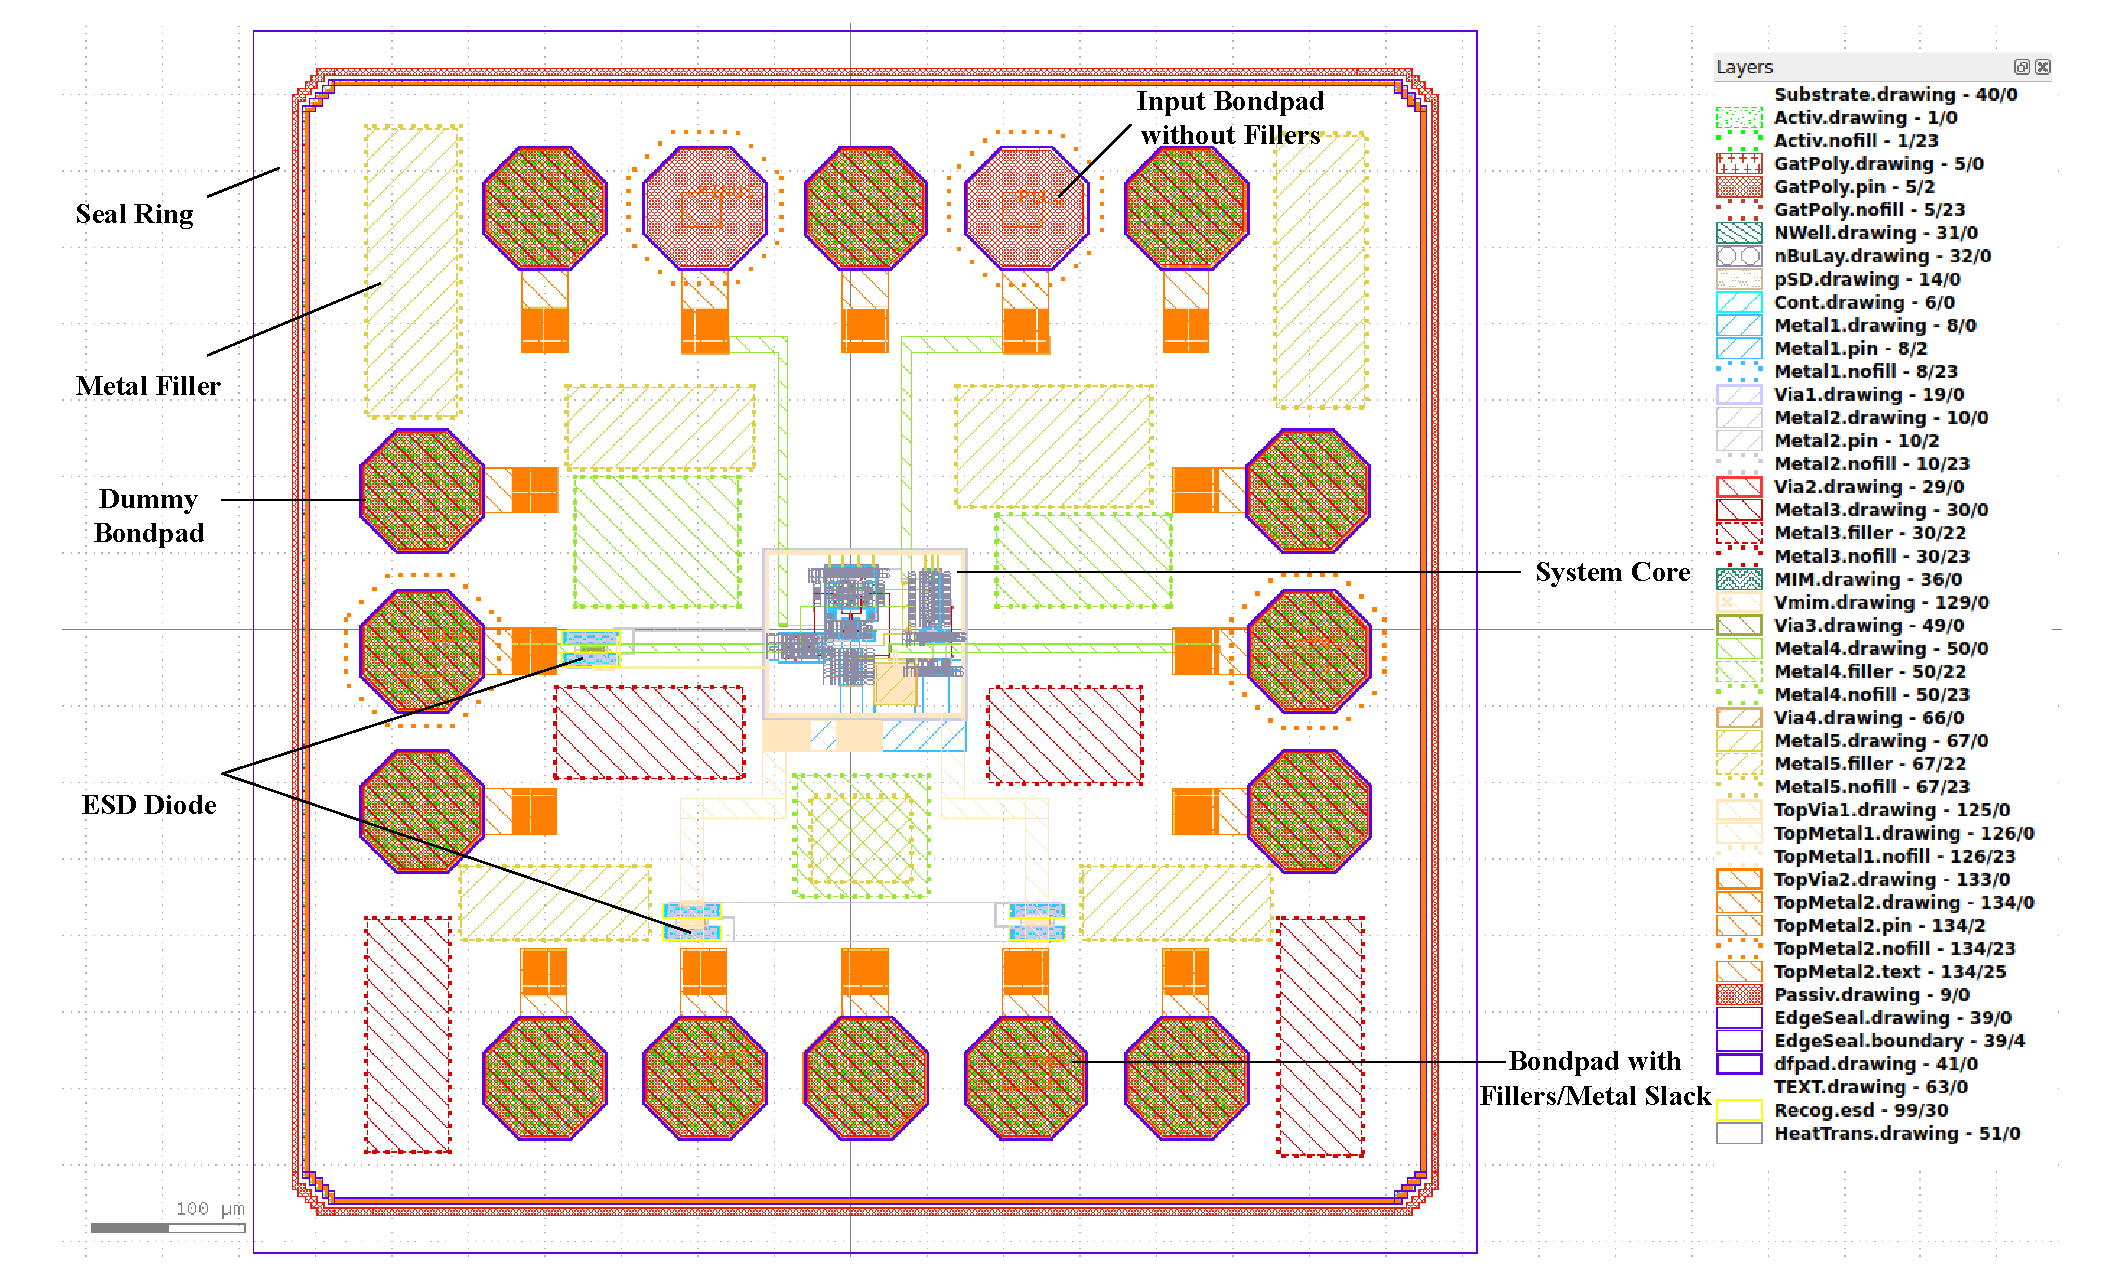
\includegraphics[width=\linewidth,height=1\textheight,keepaspectratio]{content/../figures/_fig_full_chip.pdf}

}

\caption{\label{fig-final_layout.figure}Final NMOS-OTA Chip Layout with
Bondpads, ESD Diodes and Metal Fillers around the core block before
final density fillers.}

\end{figure}%

\part{Post-Layout Simulation}

\chapter{Post layout simulation.}\label{post-layout-simulation.}

We have established testbenches for DC, AC, and transient analysis using
the symbol of the designed inverter as a subcircuit. The next step is to
perform post-layout simulation by replacing the schematic netlist with
the extracted layout netlist (PEX), in order to verify whether the
performance remains consistent after layout parasitics are included.

Firstly we need to open the symbol file in Xschem, edit the properties
of the symbol See Figure~\ref{fig-primitive}. Change from
\texttt{subcircuit} to \texttt{primitive}.

\begin{figure}[H]

\centering{

\pandocbounded{\includegraphics[keepaspectratio]{content/../figures/_fig_primitive.png}}

}

\caption{\label{fig-primitive}Primitive}

\end{figure}%

Once changed to primitive, now we can include the \texttt{.spice} file
or \texttt{.cir} file from layout to the testbench. See
Figure~\ref{fig-include}

\begin{figure}[H]

\centering{

\pandocbounded{\includegraphics[keepaspectratio]{content/../figures/_fig_include.png}}

}

\caption{\label{fig-include}Include}

\end{figure}%

Once the file is declared, we can run the testbench.

\begin{tcolorbox}[enhanced jigsaw, titlerule=0mm, bottomrule=.15mm, arc=.35mm, opacitybacktitle=0.6, colbacktitle=quarto-callout-important-color!10!white, title=\textcolor{quarto-callout-important-color}{\faExclamation}\hspace{0.5em}{Correct pin order}, coltitle=black, opacityback=0, leftrule=.75mm, left=2mm, colback=white, toptitle=1mm, breakable, bottomtitle=1mm, colframe=quarto-callout-important-color-frame, rightrule=.15mm, toprule=.15mm]

It is critically important to match the order of pins and their names.
The pin order and names in the \texttt{.cir} files need to be exact same
as included in the testbench. See the figures mentioned below

\end{tcolorbox}

\pandocbounded{\includegraphics[keepaspectratio]{content/../figures/_fig_correct_matching_xschem.png}}
\pandocbounded{\includegraphics[keepaspectratio]{content/../figures/_fig_correct_matching_cir.png}}

\textbf{Post layout and prelayout graphs to be added here as results}

\begin{figure}[H]

\centering{

\pandocbounded{\includegraphics[keepaspectratio]{index_files/mediabag/content/../figures/_fig_foldedcascode_ac_bode_postlayout.pdf}}

}

\caption{\label{fig-postlayout-output}Postlayout Results}

\end{figure}%

\chapter{PEX}\label{pex}

Parasitic Extraction (PEX) is a critical step in analog IC design that
occurs \textbf{after layout} and \textbf{before final
verification/tapeout}. It models the unintended resistive and capacitive
effects introduced by routing, device placement, and proximity in
silicon.

In analog circuits --- especially precision blocks like \textbf{folded
cascode OTAs} --- these parasitics significantly affect performance,
making PEX-based simulations essential.

\section{Why Do We Need PEX?}\label{why-do-we-need-pex}

\begin{longtable}[]{@{}
  >{\raggedright\arraybackslash}p{(\linewidth - 2\tabcolsep) * \real{0.3000}}
  >{\raggedright\arraybackslash}p{(\linewidth - 2\tabcolsep) * \real{0.7000}}@{}}
\toprule\noalign{}
\begin{minipage}[b]{\linewidth}\raggedright
Reason
\end{minipage} & \begin{minipage}[b]{\linewidth}\raggedright
Description
\end{minipage} \\
\midrule\noalign{}
\endhead
\bottomrule\noalign{}
\endlastfoot
\textbf{Performance Degradation} & Parasitic capacitance reduces
bandwidth and phase margin. \\
\textbf{Offset and Mismatch Effects} & Parasitic coupling causes
imbalance in differential paths. \\
\textbf{Stability Impact} & Additional phase lag from parasitics can
destabilize feedback loops. \\
\textbf{Post-Layout Verification} & Confirms that layout did not violate
design intent (gain, UGB, PSRR, etc.). \\
\textbf{Tapeout Confidence} & Ensures high correlation between
simulation and silicon behavior. \\
\end{longtable}

For a folded cascode OTA, RC + CC extraction is essential. It ensures
layout-induced degradation is captured early in simulation, enabling
confident tapeout. Neglecting coupling capacitance or interconnect
resistance can lead to significant performance loss or instability in
silicon.

\section{PEX using Klayout-PEX tool}\label{pex-using-klayout-pex-tool}

IIC-OSIC-Tools comes with pre-installed tool called as \textbf{K-pex}.
The current status of
\href{https://martinjankoehler.github.io/klayout-pex-website/doc/doc.html\#sec-into-klayout-pex-prototype-status}{KLayout-PEX}
says as following:

Available KLayout PEX Engines{[}9{]}:

\begin{longtable}[]{@{}
  >{\raggedright\arraybackslash}p{(\linewidth - 6\tabcolsep) * \real{0.1589}}
  >{\raggedright\arraybackslash}p{(\linewidth - 6\tabcolsep) * \real{0.1028}}
  >{\raggedright\arraybackslash}p{(\linewidth - 6\tabcolsep) * \real{0.1963}}
  >{\raggedright\arraybackslash}p{(\linewidth - 6\tabcolsep) * \real{0.5421}}@{}}
\toprule\noalign{}
\begin{minipage}[b]{\linewidth}\raggedright
Engine
\end{minipage} & \begin{minipage}[b]{\linewidth}\raggedright
PEX Type
\end{minipage} & \begin{minipage}[b]{\linewidth}\raggedright
Status
\end{minipage} & \begin{minipage}[b]{\linewidth}\raggedright
Description
\end{minipage} \\
\midrule\noalign{}
\endhead
\bottomrule\noalign{}
\endlastfoot
KPEX/MAGIC & CC, RC & Usable & Wrapper engine, using installed magic
tool \\
KPEX/FasterCap & Cp & Usable, pending QA & Field solver engine using
FasterCap \\
KPEX/FastHenry2 & R, L & Planned & Field solver engine using
FastHenry2 \\
KPEX/2.5D & CC & Under construction & Prototype engine implementing
MAGIC formulas in KLayout \\
KPEX/2.5D & R & Under construction & Prototype engine implementing MAGIC
formulas in KLayout \\
\end{longtable}

\section{\texorpdfstring{Running the
\href{https://iic-jku.github.io/klayout-pex-website/doc/doc.html\#sec-kpex-magic}{\texttt{KPEX/MAGIC}
Engine}{[}9{]}}{Running the KPEX/MAGIC Engine{[}9{]}}}\label{running-the-kpexmagic-enginekpex}

The magic section of \texttt{kpex\ -\/-help} describes the arguments and
their defaults. Important arguments:

\begin{itemize}
\tightlist
\item
  \texttt{-\/-magicrc}: specify location of the \texttt{magicrc} file\\
\item
  \texttt{-\/-gds}: path to the GDS input layout\\
\item
  \texttt{-\/-magic}: enable magic engine
\end{itemize}

\subsection{Example Command}\label{example-command}

\begin{Shaded}
\begin{Highlighting}[]
\ExtensionTok{kpex} \AttributeTok{{-}{-}pdk}\NormalTok{ ihp\_sg13g2 }\AttributeTok{{-}{-}magic} \AttributeTok{{-}{-}gds}\NormalTok{ GDS\_PATH }\AttributeTok{{-}{-}out\_dir}\NormalTok{ OUTPUT\_DIR\_PATH}
\end{Highlighting}
\end{Shaded}

more to kpex can be found under the command \texttt{kpex\ -\/-help}

\texttt{kpex\ -\/-help} command gives us the complete list of useful
commands in order to understand the usage of KPEX

Once PEX is succesfully done, the extracted netlist SPICE file will be
generated in the provided output path, which consists of extracted
parasitics which can be further used to do post layout simulations and
verify whether the design layout satisfies the design specifications or
not.

\section{Observations and Practical
Results}\label{observations-and-practical-results}

During this work, the 2025.05 Docker release of IIC-OSIC-Tools was used,
since the design was submitted on 21 August 2025, and subsequent
debugging was performed in that version. When running the FasterCap
engine, the process executed successfully; however, the generated
\texttt{.pex.spice} file was empty, indicating that no valid parasitic
data were written. Conversely, when using the MAGIC engine, a
\texttt{.pex.spice} file was generated but contained improperly scaled
parameters, leading to simulation inconsistencies.

Upon investigation of the official \href{}{IIC-OSIC-Tools release
notes}, it was confirmed that in the \texttt{2025.07} update, the
developers temporarily removed klayout-pex due to incompatibility with
several dependencies.

This subsequent removal confirms that the encountered issues in the
2025.05 environment were indeed genuine tool-level compatibility
problems, not user-level errors. Therefore, for this design, PEX-based
post-layout simulations were omitted, and circuit validation was based
on pre-layout verification complemented by manual parasitic estimation
from layout dimensions.

\bookmarksetup{startatroot}

\chapter{Conclusion}\label{conclusion}

This thesis has demonstrated that a fully open-source design flow,
combined with the IHP SG13G2 130-nm SiGe BiCMOS open PDK, is capable of
producing manufacturable analog ICs. Through the complete design and
physical implementation of a folded-cascode OTA for LED-driver control
and the successful acceptance of \textbf{two tape-outs} in the IHP
Open-MPW run of July 2025 we have shown that open-source tools can
support real mixed-signal fabrication when guided by rigorous analog
layout methodology and parasitic-conscious design practices.
Importantly, by deliberately \textbf{interchanging roles} one author
acting as circuit designer while the other served as layout engineer for
NMOS-OTA, and vice versa in the second tape-out for PMOS-OTA we gained a
comprehensive understanding of the full analog design flow, toolchain
interactions, and workflow dependencies essential for mixed-signal
development. The submitted tape-outs and supporting files can be found
in \emph{Appendix - A}. The calculated area of an individual chip is
\textbf{\(6.4 \times 10^{-7}\) sq. mm} with dimensions
\textbf{\(800\,\mu\text{m} \times 800\,\mu\text{m}\)}

The work also highlighted the strengths and current limitations of the
open ecosystem. While schematic and layout stages were executed reliably
using Xschem, Ngspice, CACE, and KLayout, parasitic extraction remains
the least mature part of the toolchain. KLayout-PEX offers preliminary
extraction capability, but a comprehensive, geometry-accurate RC
extraction and post-layout verification flow is still missing.
Strengthening open-source PEX tools should therefore be a focus of
future research, as accurate parasitic modeling is essential for
predicting analog behavior with high confidence.

Looking ahead, the fabricated chips once received, will enable full
electrical characterization. The chip will be in the form of \emph{bare
die} therefore, needs bonding. After bonding, a dedicated \textbf{PCB
test platform} should be designed to evaluate the OTA's gain, bandwidth,
bias robustness, and real-silicon parasitic effects. Such measurements
will not only validate the design but also provide deeper insight into
the accuracy and limitations of the open-source toolchain itself.

In summary, this work demonstrates that open-source analog IC design is
not only feasible but tape-out proven, while also identifying parasitic
extraction, toolchain refinement, and post-silicon testing as the key
opportunities for advancing future open-silicon research.

\bookmarksetup{startatroot}

\chapter*{Bibliography}\label{bibliography}
\addcontentsline{toc}{chapter}{Bibliography}

\markboth{Bibliography}{Bibliography}

\phantomsection\label{refs}
\begin{CSLReferences}{0}{0}
\bibitem[\citeproctext]{ref-wicht2020}
\CSLLeftMargin{{[}1{]} }%
\CSLRightInline{B. Wicht, {``Analog building blocks of dc-dc converters:
Examining fundamental concepts,''} \emph{{IEEE} Solid-State Circuits
Magazine}, vol. 12, no. 3, pp. 42--47, 2020, doi:
\href{https://doi.org/10.1109/mssc.2020.3002141}{10.1109/mssc.2020.3002141}.}

\bibitem[\citeproctext]{ref-Jespers_Murmann_2017}
\CSLLeftMargin{{[}2{]} }%
\CSLRightInline{P. G. A. Jespers and B. Murmann, \emph{Systematic design
of analog CMOS circuits: Using pre-computed lookup tables}. Cambridge
University Press, 2017.}

\bibitem[\citeproctext]{ref-pretl2024}
\CSLLeftMargin{{[}3{]} }%
\CSLRightInline{H. Pretl, M. Koefinger, and S. Dorrer, {``Analog
{Circuit} {Design}.''} Dec. 2024. doi:
\href{https://doi.org/10.5281/zenodo.14387481}{10.5281/zenodo.14387481}.}

\bibitem[\citeproctext]{ref-IHP_PDK_2024}
\CSLLeftMargin{{[}4{]} }%
\CSLRightInline{I. PDK, {``SG13G2 IHP open source layout rules,''}
Leibniz Institute for High Performance Microelectronics, Design
Reference, Dec. 2024.}

\bibitem[\citeproctext]{ref-baker2010}
\CSLLeftMargin{{[}5{]} }%
\CSLRightInline{R. J. Baker, \emph{{CMOS}: Circuit design, layout, and
simulation}, 3rd ed. Wiley-IEEE Press, 2010, p. 1208. doi:
\href{https://doi.org/10.1002/9780470891179}{10.1002/9780470891179}.}

\bibitem[\citeproctext]{ref-lienig2020}
\CSLLeftMargin{{[}6{]} }%
\CSLRightInline{J. Lienig and J. Scheible, \emph{Fundamentals of layout
design for electronic circuits}. Springer International Publishing,
2020. doi:
\href{https://doi.org/10.1007/978-3-030-39284-0}{10.1007/978-3-030-39284-0}.}

\bibitem[\citeproctext]{ref-Prof_Razavi_2001}
\CSLLeftMargin{{[}7{]} }%
\CSLRightInline{B. Razavi, \emph{Design of analog CMOS integrated
circuits}. McGraw-Hill, 2001.}

\bibitem[\citeproctext]{ref-Prof_Razavi_2011}
\CSLLeftMargin{{[}8{]} }%
\CSLRightInline{B. Razavi, \emph{Design of analog CMOS integrated
circuits}. McGraw-Hill, 2011.}

\bibitem[\citeproctext]{ref-kpex}
\CSLLeftMargin{{[}9{]} }%
\CSLRightInline{M. Köhler, {``KLayout-PEX.''} Nov. 2025. Available:
\url{https://iic-jku.github.io/klayout-pex-website/doc/doc.html}}

\end{CSLReferences}

\cleardoublepage
\phantomsection
\addcontentsline{toc}{part}{Appendices}
\appendix

\chapter{Tapeout Submissions and Repository
Links}\label{tapeout-submissions-and-repository-links}

\subsection{\texorpdfstring{\textbf{Tapeout
1}}{Tapeout 1}}\label{tapeout-1}

This design, titled \textbf{``ledamp\_ph70''}, was submitted to the
\emph{IHP Open-MPW TO\_July2025} program and is available at:\newline
\textbf{https://github.com/IHP-GmbH/TO\_July2025/tree/main/ledamp\_ph70}\newline
All associated files including the final GDSII layout, DRC reports, LVS
logs, simulation data, and documentation are provided in the
corresponding repository.\\
Tapeout 1 implements an \textbf{NMOS folded-cascode OTA}, serving as the
first realization of the analog block within the open-source flow.

\subsection{\texorpdfstring{\textbf{Tapeout
2}}{Tapeout 2}}\label{tapeout-2}

The second submission, titled \textbf{``OTALED''}, is hosted
at:\newline 
\textbf{https://github.com/IHP-GmbH/TO\_July2025/tree/main/OTALED}\\
This repository contains the complete set of fabrication-ready
deliverables, analogous to Tapeout\_1: layout, verification reports,
extracted netlists, and supporting documentation.\\
In contrast to Tapeout 1, Tapeout 2 implements a \textbf{PMOS
folded-cascode OTA}, enabling a comparative evaluation of device
polarity, layout strategies, and biasing considerations within the same
SG13G2 process.

Together, these two tapeouts document the full analog design cycle
executed twice with interchanged roles, providing a complete
methodological reference for future open-source mixed-signal tapeout
efforts.

\chapter{Final Chip Layout}\label{final-chip-layout}

\begin{figure}[H]

\centering{

\includegraphics[width=\linewidth,height=1\textheight,keepaspectratio]{content/../figures/_fig_PMOS_with_fillers.pdf}

}

\caption{\label{fig-pmos}Final PMOS OTA after adding fillers}

\end{figure}%

\chapter{USB-Stick and Script
Referencing}\label{usb-stick-and-script-referencing}

All directory structures and file paths presented in this appendix are
intentionally simplified. They are provided to clarify the organization
of the project and to indicate where specific scripts, netlists,
verification outputs, and layout files can be found within the design
environment.

\begin{Shaded}
\begin{Highlighting}[]
\NormalTok{thesis\_hp/}
\NormalTok{├── .gitattributes}
\NormalTok{├── .gitignore}
\NormalTok{├── \_book/}
\NormalTok{├── \_quarto/}
\NormalTok{├── \_quarto.yml}
\NormalTok{├── \_bibliography}
\NormalTok{├── \_manuscript}
\NormalTok{├── index.qmd             \# Main project page / Abstract}
\NormalTok{├── README.md}
\NormalTok{├── references.qmd}
\NormalTok{├── KNOWN\_ISSUES.md}
\NormalTok{├── cace/                 \# CACE setup for corner alaysis, PVT, MonteCarlo.}
\NormalTok{├── content/              \# contains all the .qmd files for documentation}
\NormalTok{├── Designs/              \# Top{-}level Design Folder}
\NormalTok{│   ├── 1\_schematics/     \# (Design subfolder: Circuit schematics)}
\NormalTok{        ├── otas/          \# contains .sch files of otas}
\NormalTok{│   ├── 2\_layout/         \# (Design subfolder: Physical layout files)}
\NormalTok{        ├── tapeout/}
\NormalTok{            ├── final\_layout\_before\_fillering/   \# final gds files}
\NormalTok{│   └── 3\_kpex/           \# (Design subfolder: Extracted parasitic netlists)}
\NormalTok{├── Expose\_HP/            }
\NormalTok{├── figures/              \# contains all the figues for documentation}
\NormalTok{├── layout\_scripts/       \# DRC Error Check and Minimum Finger Estimation scripts}
\NormalTok{├── Literature/           \# References or literature review material}
\NormalTok{├── python\_codes/         \# Python scripts to plot raw data}
\NormalTok{├── sizing/}
\NormalTok{    ├── matlab/            \# contains matlab codes for lookup tables }
\NormalTok{    ├── python/            \# sizing using pygmid tool and python scripts for sizing}
\NormalTok{    ├── xschem/            \# contains testbenches on mosfets to Extract data  }
\NormalTok{                          \# provided by foundry to use them for gm id method}
\NormalTok{├── simulations/          \# Folder for .spice files and .raw outputs}
\NormalTok{└── postlayout\_simulations/   \# Post{-}Layout Simulation results/setup}
\end{Highlighting}
\end{Shaded}



\backmatter


\end{document}
